\documentclass[12pt]{article}
\usepackage{rotating}
\usepackage{amssymb, amsmath, amsthm, graphicx} 
\usepackage{multirow}
\usepackage{setspace}
\usepackage{enumerate}
\usepackage{graphicx}
\usepackage{listings}
\usepackage{multirow}
\usepackage{color}
\usepackage{threeparttable}
\usepackage{caption}
\usepackage{subcaption}
\usepackage{todonotes}
\usepackage{mathrsfs}
\usepackage[margin=1.2in]{geometry}
	
\usepackage{setspace}
% \singlespacing
\onehalfspacing
% \doublespacing
% \setstretch{<factor>} % for custom spacing

\RequirePackage{natbib}
\RequirePackage[colorlinks]{hyperref}
\RequirePackage{hypernat}


\newcommand{\p}{\mathbb{P}}
\DeclareMathOperator*{\argmin}{arg\,min}

\newtheorem{assump}{Assumption}[section]
\newtheorem{pro}{Proposition}[section]
\newtheorem{lem}{Lemma}[section]
\newtheorem{thm}{Theorem}[section]
\newtheorem{cor}{Corollary}[section]
\newtheorem{ineq}{Inequality}[section]
\newtheorem{defn}{Definition}[section]
\newtheorem{rem}{Remark}[section]
\newtheorem{ex}{Example}[section]
\theoremstyle{definition}
\newtheorem{alg}{Algorithm}[section]

%Bold proof titles
\makeatletter \renewenvironment{proof}[1][\proofname] {\par\pushQED{\qed}\normalfont\topsep6\p@\@plus6\p@\relax\trivlist\item[\hskip\labelsep\bfseries#1\@addpunct{.}]\ignorespaces}{\popQED\endtrivlist\@endpefalse} \makeatother



\begin{document}



\title{Using Invalid Instruments on Purpose: Focused Moment Selection and Averaging for GMM\footnote{I thank Aislinn Bohren, Gerda Claeskens, Bruce Hansen, Byunghoon Kang, Toru Kitagawa, Hannes Leeb, Serena Ng, Alexei Onatski, Hashem Pesaran, Benedikt P\"{o}tscher, Frank Schorfheide, Neil Shephard,  Richard J.\ Smith, Stephen Thiele, Melvyn Weeks, as well as seminar participants at Cambridge, the University of Vienna, Queen Mary, St Andrews, George Washington, UPenn, Columbia, Oxford, and the 2011 Econometric Society European Meetings for their many helpful comments and suggestions. I thank Kai Carstensen for providing data for my empirical example.}}

\author{Francis J.\ DiTraglia \\ University of Pennsylvania}

\date{\normalsize First Version: November 15, 2011 \\ This Version: \today}

\maketitle 
\begin{abstract}
In finite samples, the use of a slightly endogenous but highly relevant instrument can reduce mean-squared error (MSE). Building on this observation, I propose a moment selection criterion for GMM in which over-identifying restrictions are chosen based on the MSE of their associated estimators rather than their validity: the focused moment selection criterion (FMSC). I then show how the framework used to derive the FMSC can address the problem of inference post-moment selection. Treating post-selection estimators as a special case of moment-averaging, in which estimators based on different moment sets are given data-dependent weights, I propose a simulation-based procedure to construct valid confidence intervals. In a Monte Carlo experiment, the FMSC outperforms alternatives suggested in the literature, and the simulation-based procedure achieves its stated minimum coverage. I conclude with an empirical example examining the effect of instrument selection on the estimated relationship between malaria transmission and economic development.
\end{abstract}
%Wordcount: 148




\section{Introduction}
%For consistent estimates, instrumental variables must be exogenous and relevant: correlated with the endogenous regressors but uncorrelated with the error term.

In finite samples, the use of an endogenous but sufficiently relevant instrument can improve inference, reducing estimator variance by far more than bias is increased. 
Building on this observation, I propose a new moment selection criterion for generalized method of moments (GMM) estimation: the focused moment selection criterion (FMSC). 
Rather than selecting only valid moment conditions, the FMSC chooses from a set of potentially mis-specified moment conditions to yield the smallest mean squared error (MSE) GMM estimator of a user-specified target parameter. 
I derive FMSC using asymptotic mean squared error (AMSE) to approximate finite-sample MSE. To ensure that AMSE remains finite, I employ a drifting asymptotic framework in which mis-specification, while present for any fixed sample size, vanishes in the limit. 
In the presence of such \emph{locally mis-specified} moment conditions, GMM remains consistent although, centered and rescaled, its limiting distribution displays an asymptotic bias. Adding an additional mis-specified moment condition introduces a further source of bias while reducing asymptotic variance. 
The idea behind FMSC is to trade off these two effects in the limit as an approximation to finite sample behavior. 
%While estimating asymptotic variance is straightforward, even under local mis-specification, estimating asymptotic bias requires over-identifying information. 
I consider a setting in which two blocks of moment conditions are available: one that is assumed correctly specified, and another that may not be.
When the correctly specified block identifies the model, I derive an asymptotically unbiased estimator of AMSE: the FMSC. When this is not the case, it remains possible to use the AMSE framework to carry out a sensitivity analysis. 
\todo[inline]{Should relate this to Andrews-style papers as well as Liao and Cheng.}

Continuing under the local mis-specification assumption, I show how the ideas used to derive FMSC can be applied to the important problem of inference post-moment selection. 
Because they use the same data twice, first to choose a moment set and then to carry out estimation, post-selection estimators are randomly weighted averages of many individual estimators.
While this is typically ignored in practice, its effects can be dramatic: coverage probabilities of traditional confidence intervals are generally far too low, even for consistent moment selection. 
I treat post-selection estimators as a special case of moment averaging: combining estimators based on different moment sets with data-dependent weights.
By deriving the limiting distribution of moment average estimators, I propose a simulation-based procedure for constructing valid confidence intervals. This technique can be applied to moment averaging and post-selection estimators based on a variety of criteria including FMSC. 

While the methods described here apply to any model estimated by GMM, subject to standard regularity conditions, I focus on their application to linear instrumental variables (IV) models. 
In simulations for two-stage least squares (2SLS), FMSC performs well relative to alternatives suggested in the literature. 
Further, the procedure for constructing valid confidence intervals achieves its stated minimum coverage, even in situations where instrument selection leads to highly non-normal sampling distributions. 
I conclude with an empirical application from development economics, exploring the effect of instrument selection on the estimated relationship between malaria transmission and income. 

My approach to moment selection under mis-specification is inspired by the focused information criterion of \citet{ClaeskensHjort2003}, a model selection criterion for models estimated by maximum likelihood. 
Like them, I allow for mis-specification and use AMSE to approximate small-sample MSE in a drifting asymptotic framework. 
In contradistinction, however, I consider moment rather than model selection, and general GMM estimation rather than maximum likelihood.
 
The existing literature on moment selection under mis-specification is comparatively small. 
\cite{Andrews1999} proposes a family of moment selection criteria for GMM by adding a penalty term to the J-test statistic. 
Under an identification assumption and certain restrictions on the form of the penalty, these criteria consistently select all correctly specified moment conditions in the limit. 
\cite{AndrewsLu} extend this work to allow simultaneous GMM moment and model selection, while \cite{HongPrestonShum} derive analogous results for generalized empirical likelihood. 
More recently, \cite{Liao} proposes a shrinkage procedure for simultaneous GMM moment selection and estimation. 
Given a set of correctly specified moment conditions that identifies the model, this method consistently chooses all valid conditions from a second set of potentially mis-specified conditions.
In contrast to these proposals, which examine only the validity of the moment conditions under consideration, the FMSC balances validity against relevance to minimize MSE. 
The only other proposal from the literature to consider both validity and relevance in moment selection is a suggestion by \cite{HallPeixe2003} to combine their canonical correlations information criterion (CCIC) -- a relevance criterion that seeks to avoid including redundant instruments -- with Andrews' GMM moment selection criteria. 
This procedure, however, merely seeks to avoid including redundant instruments after eliminating invalid ones: it does not allow for the intentional inclusion of a slightly invalid but highly relevant instrument to reduce MSE. 


The idea of choosing instruments to minimize MSE is shared by the procedures in \cite{DonaldNewey2001} and \cite{DonaldImbensNewey2009}. 
\cite{KuersteinerOkui2010} also aim to minimize MSE but, rather than choosing a particular instrument set, suggest averaging over the first-stage predictions implied by many instrument sets and using this average in the second stage. 
Unlike FMSC, these papers consider the higher-order bias that arises from including many valid instruments rather than the first-order bias that arises from the use of invalid instruments.

The literature on post-selection, or ``pre-test'' estimators is vast. \citet{LeebPoetscher2005, LeebPoetscher2009}  give a theoretical overview, while \cite{Demetrescu} illustrate the practical consequences via a simulation experiment. There are several proposals to construct valid confidence intervals post-model selection, including \cite{Kabaila1998}, \cite{HjortClaeskens} and \cite{KabailaLeeb2006}. 
To my knowledge, however, this is the first paper to examine the problem specifically from the perspective of moment selection. The approach adopted here, treating post-moment selection estimators as a specific example of moment averaging, is adapted from the frequentist model average estimators of \cite{HjortClaeskens}.
Another paper that considers weighting GMM estimators based on different moment sets is \cite{Xiao}. While Xiao combines estimators based on valid moment conditions to achieve a minimum variance estimator, I combine estimators based on potentially invalid conditions to minimize MSE. 
A similar idea underlies the combined moments (CM) estimator of \cite{Judge2007}, who emphasize that incorporating the information from an incorrect specification could lead to favorable bias-variance tradeoff. 
%Their proposal uses a Cressie-Read divergence measure to combine the information from competing moment specifications, for example OLS versus two-stage least squares (2SLS), yielding a data-driven compromise estimator. Unlike the FMSC, however, the CM estimator is not targeted to a particular research goal and does not explicitly aim to minimize MSE.

The remainder of the paper is organized as follows.
Section \ref{sec:asymp} describes the local mis-specification framework and gives the main limiting results used later in the paper. 
Section \ref{sec:FMSC} derives FMSC as an asymptotically unbiased estimator of AMSE, presents specialized results for 2SLS, and examines their performance in a Monte Carlo experiment. 
Section \ref{sec:avg} describes a simulation-based procedure to construct valid confidence intervals for moment average estimators and examines its performance in a Monte Carlo experiment. Section \ref{sec:application} presents the empirical application and Section \ref{sec:conclude} concludes. 
Proofs appear in the Appendix.

\todo[inline]{Final step: rewrite abstract and intro. Main additions: (1) Add some of the additional refsthat the referees suggested, (2) Add some further refs backing up my approach and some more recent FIC-style work, (3) mention the limitation of strong identification but try to suggest that the simulation studies partially address this, (4) stress large gains to be had from using this procedure. Most importantly, try to make it clear why I'm doing conservative/efficient model selection rather than consistent model selection. Refer to the Hansen shrinkage paper?}
 

\section{Assumptions and Asymptotic Framework}
\label{sec:asymp}

\subsection{Local Mis-Specification}
Let $f(\cdot,\cdot)$ be a $(p+q)$-vector of moment functions of a random vector $Z$ and an $r$-dimensional parameter vector $\theta$, partitioned according to $f(\cdot,\cdot) = \left(g(\cdot,\cdot)', h(\cdot,\cdot)'  \right)'$ where $g(\cdot,\cdot)$ and $h(\cdot,\cdot)$ are $p$- and $q$-vectors of moment functions. 
The moment condition associated with $g(\cdot,\cdot)$ is assumed to be correct whereas that associated with $h(\cdot,\cdot)$ is locally mis-specified.
More precisely, 
\begin{assump}[Local Mis-Specification]
\label{assump:drift}
Let $\{Z_{ni}\colon 1\leq i \leq n, n =1, 2, \hdots\}$ be a triangular array of random vectors defined on a probability space $(\Upsilon, \mathcal{F}, \p)$ satisfying
	\begin{enumerate}[(a)]
		\item $E[g(Z_{ni},\theta_0)] = 0$,
		\item $E[h(Z_{ni},\theta_0)] = n^{-1/2}\tau$, where $\tau$ is an unknown constant vector, 
		\item $\{f(Z_{ni},\theta_0)\colon 1\leq i \leq n, n = 1, 2, \hdots\}$ is uniformly integrable, and
		\item $Z_{ni} \rightarrow_dZ_i$, where the $Z_i$ are identically distributed.
	\end{enumerate}
\end{assump}
For any fixed sample size $n$, the expectation of $h$ evaluated at the true parameter value value $\theta_0$ depends on the unknown constant vector $\tau$. 
Unless all components of $\tau$ are zero, some of the moment conditions contained in $h$ are mis-specified. In the limit however, this mis-specification vanishes, as $\tau/\sqrt{n}$ converges to zero. 
Uniform integrability combined with weak convergence implies convergence of expectations, so that $E[g(Z_i, \theta_0)]=0$ and $E[h(Z_i, \theta_0)]=0$. Because the limiting random vectors $Z_i$ are identically distributed, we suppress the $i$ subscript and simply write $Z$ to denote their common marginal law, e.g.\ $E[h(Z,\theta_0)]=0$. 
It is important to note that local mis-specification is \emph{not} intended as a literal description of real-world datasets: it is merely a device that gives asymptotic bias-variance trade-off that mimics the finite-sample intuition. 

\subsection{Candidate GMM Estimators}
Define the sample analogue of the expectations in Assumption \ref{assump:drift} as follows:
$$f_n(\theta) = \frac{1}{n}\sum_{i=1}^n f(Z_{ni},\theta) = \left[\begin{array}{c} g_n(\theta)\\ h_n(\theta) \end{array} \right]=\left[\begin{array}{c}n^{-1}\sum_{i=1}^n g(Z_{ni},\theta) \\ n^{-1}\sum_{i=1}^n h(Z_{ni},\theta) \end{array}\right]$$
where $g_n$ is the sample analogue of the correctly specified moment conditions and $h_n$ is that of the (potentially) mis-specified moment conditions.
A candidate GMM estimator $\widehat{\theta}_S$ uses some subset $S$ of the moment conditions contained in $f$ in estimation. 
Let $|S|$ denote the number of moment conditions used. For $\widehat{\theta}_S$ to be identified, we require that $|S|>r$. 
Let $\Xi_S$ be the $|S| \times(p +q)$ \emph{moment selection matrix} corresponding to $S$. That is, $\Xi_S$ is a matrix of ones and zeros arranged such that $\Xi_S f_n(\theta)$ contains only the sample moment conditions used to estimate $\widehat{\theta}_S$. 
Thus, the GMM estimator of $\theta$ based on moment set $S$ is given by 
$$\widehat{\theta}_S = \argmin_{\theta \in \Theta}\; \left[\Xi_S f_n(\theta)\right]' \widetilde{W}_S \; \left[ \Xi_S f_n(\theta)\right].$$
where $\widetilde{W}_S$ is an $|S|\times |S|$, positive semi-definite weight matrix. Note that we place no restrictions on $S$ other than $|S| >r$ so that the estimator exists. 
In particular, $S$ may \emph{exclude} some or all of the valid moment conditions contained in $g$.
While this may seem strange, it allows us to accomodate a wider range of examples, including choosing between least squares and instrumental variables estimators.

To consider the limit distribution of $\widehat{\theta}_S$, we require some further notation. 
First define the derivative matrices
	$$G = E\left[\nabla_{\theta} \; g(Z,\theta_0)\right], \quad H = E\left[\nabla_{\theta} \; h(Z,\theta_0)\right], \quad F = (G', H')'$$
and let $\Omega = Var\left[ f(Z,\theta_0) \right]$ where $\Omega$ is partitioned into blocks $\Omega_{gg}$, $\Omega_{gh}$, $\Omega_{hg}$, and $\Omega_{hh}$ conformably with the partition of $f$ by $g$ and $h$. 
Notice that each of these expressions involves the \emph{limiting random variable} $Z$ rather than $Z_{ni}$, so that the corresponding expectations are taken with respect to a distribution for which all moment conditions are correctly specified. 
Finally, to avoid repeatedly writing out pre- and post-multiplication by $\Xi_S$, define $F_S = \Xi_S F$ and $\Omega_S = \Xi_S \Omega\Xi_S'$. 
The following high level assumptions are sufficient for the consistency and asymptotic normality of the candidate GMM estimator $\widehat{\theta}_S$. 
\begin{assump}[High Level Sufficient Conditions]
\label{assump:highlevel} 
\mbox{}
	\begin{enumerate}[(a)]
		\item $\theta_0$ lies in the interior of $\Theta$, a compact set
		\item $\widetilde{W}_S \rightarrow_{p} W_S$, a positive definite matrix
		\item $W_S \Xi_S E[f(Z,\theta)]=0$ if and only if $\theta = \theta_0$
		\item $E[f(Z,\theta)]$ is continuous on $\Theta$
		\item $\sup_{\theta \in \Theta}\| f_n(\theta)- E[f(Z,\theta)]\|\rightarrow_{p} 0$
		\item $f$ is Z-almost surely differentiable in an open neighborhood $\mathcal{B}$ of $\theta_0$
		\item $\sup_{\theta \in \Theta} \|\nabla_{\theta}f_n(\theta) - F(\theta)\|\rightarrow_{p} 0$
		\item $\sqrt{n}f_n(\theta_0) \rightarrow_d  M + \left[\begin{array}{c}0\\ \tau \end{array} \right]$ where $M \sim N_{p+q}\left(0, \Omega \right)$
		\item $F_S'W_SF_S$ is invertible
	\end{enumerate}
\end{assump}

Although Assumption \ref{assump:highlevel} closely approximates the standard regularity conditions for GMM estimation, establishing primitive conditions for Assumptions \ref{assump:highlevel} (d), (e), (g) and (h) is slightly more involved under local mis-specification. 
Low-level sufficient conditions for the two running examples considered in this paper appear in Sections \ref{sec:OLSvsIVlowlevel} and  \ref{sec:chooseIVlowlevel} below. 
For more general results, see \cite{Andrews1988} Theorem 2 and \cite{Andrews1992} Theorem 4.  
Notice that identification, (c), and continuity, (d), are conditions on the distribution of $Z$, the marginal law to which each $Z_{ni}$ converges. 

\begin{thm}[Consistency]
\label{thm:consist}
Under Assumptions \ref{assump:drift} and \ref{assump:highlevel} (a)--(e), $\widehat{\theta}_S \rightarrow_{p} \theta_0$.
\end{thm}

\begin{thm}[Asymptotic Normality]
\label{thm:normality}
Under Assumptions \ref{assump:drift} and \ref{assump:highlevel}
$$\sqrt{n}(\widehat{\theta}_S - \theta_0 ) \rightarrow_d -K_S \Xi_S  \left(\left[\begin{array}
	{c} M_g \\ M_h
\end{array} \right]  + \left[\begin{array}
	{c} 0 \\ \tau
\end{array} \right]\right)$$
where $K_S  = [F_S'W_SF_S]^{-1} F_S'W_S$, $M = (M_g', M_h')'$, and $M \sim N(0,\Omega)$.
\end{thm}

As we see from Theorems \ref{thm:consist} and \ref{thm:normality}, \emph{any} candidate GMM estimator $\widehat{\theta}_S$ is consistent for $\theta_0$ under local mis-specification. 
Unless $S$ excludes \emph{all} of the moment conditions contained in $h$, however, $\widehat{\theta}_S$ inherits an asymptotic bias from the mis-specification parameter $\tau$. 
The local mis-specification framework is useful precisely because it results in a limit distribution for $\widehat{\theta}_S$ with both a bias \emph{and} a variance. 
This captures in asymptotic form the bias-variance tradeoff that we see in finite sample simulations.
In constrast, fixed mis-specification results in a degenerate bias-variance tradeoff in the limit: scaling up by $\sqrt{n}$ to yield an asymptotic variance causes the bias component to diverge.

\subsection{Identification}
Any form of moment selection requires an identifying assumption: we need to make clear which parameter value $\theta_0$ counts as the ``truth.''
One approach, following \cite{Andrews1999}, is to assume that there exists a unique, maximal set of correctly specified moment conditions that identifies $\theta_0$. 
In the notation of the present paper\footnote{Although \cite{Andrews1999}, \cite{AndrewsLu}, and \cite{HongPrestonShum} consider \emph{fixed} mis-specification, we can view this as a version of local mis-specification in which $\tau \rightarrow \infty$.} this is equivalent to the following:

\begin{assump}[\cite{Andrews1999} Identification Condition]
	\label{assump:Andrews}
There exists a subset $S_{max}$ of at least $r$ moment conditions satisfying:
	\begin{enumerate}
	 	\item $\Xi_{S_{max}} E[f(Z_{ni},\theta_0)]= 0$
	 	\item For any $S' \neq S_{max}$ such that $\Xi_{S'} E[f(Z_{ni},\theta')]= 0$ for some $\theta' \in \Theta$, $|S_{max}| > |S'|$.
	 \end{enumerate}
\end{assump}

\cite{AndrewsLu} and \cite{HongPrestonShum} take the same basic approach to identification, with appropriate modifications to allow for simultaneous model and moment selection. 
An advantage of Assumption \ref{assump:Andrews} is that, under fixed mis-specification, it allows consistent selection of $S_{max}$ without any prior knowledge of \emph{which} moment conditions are correct. 
In the notation of the present paper this corresponds to having no moment conditions in the $g$ block. As \citet[p.\ 254]{Hallbook} points out, however, the second part of Assumption \ref{assump:Andrews} can fail even in simple settings such as linear instrumental variables estimation. 
When it does fail, the selected GMM estimator may no longer be consistent for $\theta_0$. 

A different approach to identification is to assume that there is a minimal set of at least $r$ moment conditions \emph{known} to be correctly specified.
This is the approach we follow here, one shared by \cite{Liao} and \cite{ChengLiao}. 
With the exception of Section \ref{subsec:digress}, we maintain the following assumption throughout.

\begin{assump}[FMSC Identification Condition] 
\label{assump:Identification}
Let $\widehat{\theta}_v$ denote the GMM estimator based solely on the moment conditions contained in the $g$--block
$$\widehat{\theta}_v = \argmin_{\theta \in \Theta}\; g_n(\theta)' \widetilde{W}_{v} \; g_n(\theta)$$
We call this the ``valid estimator'' and assume that it is identified, i.e.\ that $p\geq r$.
\end{assump}

Assumption \ref{assump:Identification} and Theorem \ref{thm:normality} immediately imply that the valid estimator shows no asymptotic bias. 
For convenience, we state its limit distribution in the following Corollary: 
\begin{cor}[Limit Distribution of Valid Estimator]
	\label{cor:valid}
	Let $S_{v}$ include only the moment conditions contained in $g$. 
	Then, under Assumption \ref{assump:Identification} we have
		$$\sqrt{n}\left(\widehat{\theta}_v - \theta_0\right) \rightarrow_d -K_v M_g$$
	by applying Theorem \ref{thm:normality} to $S_{v}$, where $K_v = [G'W_vG]^{-1}G'W_v$ and $M_g \sim N(0,\Omega_{gg})$. 
\end{cor}

Both Assumptions \ref{assump:Andrews} and \ref{assump:Identification} are strong, and neither fully nests the other. 
Which should be preferred is both a matter of taste and of the particular application one has in mind.
In the context of the present paper, Assumption \ref{assump:Identification} is meant to represent a situation that is common in empirical practice. 
The $g$--block of moment conditions contains the ``baseline'' assumptions that an empirical researcher would be prepared to defend in a seminar, while the $h$--block represents a set of stronger, more controversial assumptions. 
In the FMSC framework, moment selection is carried out \emph{conditional} on the baseline assumptions: we use the $g$--block to help us decide whether to include any of the moment conditions contained in the $h$--block. 
But why would we ever consider using controversial assumptions? 
FMSC is designed for settings in which the $h$--block is expected to contain a substantial amount of information beyond that already contained in the $g$--block. 
The idea is that, if we knew the $h$--block was correctly specified, we would expect a large gain in efficiency by including it in estimation. 
This motivates the idea of trading off the variance reduction from including $h$ against the potential increase in bias. 
Not all applications have the structure, but many important ones do. 
We now consider two motivating examples. 



\subsection{Example: OLS versus 2SLS}
\label{sec:OLSvsIVlowlevel}
The simplest interesting application of the FMSC is choosing between ordinary least squares (OLS) and two-stage least squares (2SLS) estimators of the effect $\beta$ of a single endogenous regressor $x$ on an outcome of interest $y$. 
To keep the presentation transparent, we will work within an iid, homoskedastic setting. 
Neither of these restrictions, however, is necessary. 
Without loss of generality we may assume that there are no exogenous regressors, or equivalently that they have been ``projected out of the system,'' so that the data generating process is given by
    \begin{eqnarray}
			y_{i} &=& \beta x_{i}  + \epsilon_{i}\\
	x_{i} &=& \mathbf{z}_{i}' \boldsymbol{\pi} + v_{i}
	\end{eqnarray}
where $\beta$ and $\boldsymbol{\pi}$ are unknown constants, $\mathbf{z}_i$ is a vector of exogenous and relevant instruments, $x_i$ is the endogenous regressor, $y_i$ is the outcome of interest, and $\epsilon_i, v_i$ are unobservable error terms. 
All random variables in this system are mean zero, or equivalently all constant terms have been projected out. 
Stacking observations in the usual way, let 
$\mathbf{z}' = (z_{1}, \hdots, z_{n})$, $Z' = (\mathbf{z}_{1}, \hdots, \mathbf{z}_{n})$, $\mathbf{x}' = (x_{1}, \hdots, x_{n})$ and so on. The two estimators under consideration are the OLS estimator $\widehat{\beta}_{OLS}$ and the 2SLS estimator $\widetilde{\beta}_{2SLS}$
  \begin{eqnarray} 
  \label{eq:OLS}
		\widehat{\beta}_{OLS} &=& \left(\mathbf{x}'\mathbf{x}\right)^{-1}\mathbf{x}'\mathbf{y}\\
	\label{eq:2SLS}
		\widetilde{\beta}_{2SLS} &=& \left(\mathbf{x}'P_Z\mathbf{x}\right)^{-1}\mathbf{x}'P_Z\mathbf{y}
	\end{eqnarray}
where $P_Z = Z(Z'Z)^{-1}Z'$. 
But why should we even \emph{consider} using OLS if $x$ is endogenous and we have valid instruments at our disposal? 
The answer is simple: 2SLS is a high variance estimator. 
Depending on the degree of endogeneity present in $x$ and the strength of the instruments, $\widehat{\beta}_{OLS}$ could easily have the lower mean-squared error of the two estimators.
\footnote{Because the moments of the 2SLS estimator only exist up to the order of overidentificiation \citep{Phillips1980} this statement should be understood to refer to ``trimmed'' mean-squared error when the number of instruments is two or fewer. For more discussion of this point, see the simulation results below.} 
We can embed this intuition within the local mis-specification framework as follows
  \begin{equation}
     E \left[\begin{array}{c} \mathbf{z}_{ni} \epsilon_{ni} \\ x_{ni} \epsilon_{ni} \end{array}\right] = \left[\begin{array}{c} \mathbf{0} \\ \tau/\sqrt{n} \end{array}\right].
  \end{equation}
where $\mathbf{0}$ is a vector of zeros, and $\tau$ is an unknown constant that encodes the endogeneity of $\tau$. 
In this setting, there is only a single moment condition in the $h$--block: $E[x_{ni}\epsilon_{ni}] = \tau/\sqrt{n}$. 
The question is not whether we should use this moment condition \emph{in addition} to the 2SLS moment conditions written above it, but rather whether we should use it \emph{instead} of them.
The following simple low-level conditions are sufficient for the asymptotic normality of the OLS and 2SLS estimators in this example.

\begin{assump}[OLS versus 2SLS]\label{assump:OLSvsIV}
	Let $\{(\mathbf{z}_{ni}, v_{ni}, \epsilon_{ni})\colon 1\leq i \leq n, n = 1, 2, \hdots\}$ be a triangular array of random variables such that
	\begin{enumerate}[(a)]
		\item $(\mathbf{z}_{ni}, v_{ni}, \epsilon_{ni}) \sim$ iid and mean zero within each row of the array (i.e.\ for fixed $n$)
		\item $E[\mathbf{z}_{ni} \epsilon_{ni}]=\mathbf{0}$, $E[\mathbf{z}_{ni} v_{ni}]=\mathbf{0}$, and $E[\epsilon_{ni}v_{ni}] = \tau/\sqrt{n}$ for all $n$
		\item $E[\left|\mathbf{z}_{ni}\right|^{4+\eta}] <C$, $E[\left|\epsilon_{ni}\right|^{4+\eta}] <C$, and $E[\left|v_{ni}\right|^{4+\eta}] <C$ for some $\eta >0$, $C <\infty$
		\item $E[\mathbf{z}_{ni} \mathbf{z}_{ni}'] \rightarrow Q>0$, $E[v_{ni}^2]\rightarrow \sigma_v^2 >0$, and $E[\epsilon_{ni}^2] \rightarrow \sigma_\epsilon^2 >0$ as $n\rightarrow \infty$
		\item As $n\rightarrow \infty$, $E[\epsilon_{ni}^2 \mathbf{z}_{ni} \mathbf{z}_{ni}']- E[\epsilon_{ni}^2]E[ \mathbf{z}_{ni} \mathbf{z}_{ni}'] \rightarrow 0$, $E[\epsilon_i^2 v_{ni} \mathbf{z}_{ni}'] - E[\epsilon_{ni}^2]E[v_{ni} \mathbf{z}_{ni}'] \rightarrow 0$, and $E[\epsilon_{ni}^2 v_{ni}^2] - E[\epsilon_{ni}^2]E[v_{ni}^2] \rightarrow 0$
		\item $x_{ni} = \mathbf{z}_{ni}'\boldsymbol{\pi} + v_i$ where $\boldsymbol{\pi} \neq \mathbf{0}$, and $y_{ni} = \beta x_{ni} + \epsilon_{ni}$
	\end{enumerate}
\end{assump}

Parts (a), (b) and (d) correspond to the local mis-specification assumption, part (c) is a set of moment restrictions, and (f) is simply the DGP.
Part (e) is the homoskedasticity assumption: an \emph{asymptotic} restriction on the joint distribution of $v_{ni}$, $\epsilon_{ni}$, and $\mathbf{z}_{ni}$. 
This condition holds automatically, given the other asssumptions, if $(\mathbf{z}_{ni}, v_{ni}, \epsilon_{ni})$ are jointly normal, as in our simulation experiment described below. 

\begin{thm}[OLS and 2SLS Limit Distributions]
	\label{thm:OLSvsIV} Under Assumption \ref{assump:OLSvsIV},
	$$
\left[
\begin{array}{c}
  \sqrt{n}(\widehat{\beta}_{OLS} - \beta) \\
  \sqrt{n}(\widetilde{\beta}_{2SLS} - \beta)
\end{array}
\right] \overset{d}{\rightarrow}
N\left(
\left[
\begin{array}{c}
\tau/\sigma_x^2 \\ 
0
\end{array}
\right],\;
\sigma_\epsilon^2 \left[ \begin{array}{cc}
  1/\sigma_x^2 & 1/\sigma_x^2\\
  1/\sigma_x^2 & 1/\gamma^2 
  \end{array}\right]
  \right)
$$
where $\sigma_x^2 = \gamma^2 + \sigma_v^2$, $\gamma^2 = \boldsymbol{\pi}'Q \boldsymbol{\pi}$, and $Q$, $ \sigma_\epsilon^2$, and $\sigma_v^2$ are defined in Assumption \ref{assump:OLSvsIV}.
\end{thm}

We see from the preceding result that the variance of the OLS estimator is always strictly lower than that of the 2SLS estimator since $\sigma^2_\epsilon/\sigma_x^2 = \sigma^2_\epsilon/(\gamma^2 + \sigma_v^2)$. 
Unless $\tau = 0$, however, OLS shows an asymptotic bias. 
In contrast, the 2SLS estimator is asymptotically unbiased regardless of the value of $\tau$.  



\subsection{Example: Choosing Instrumental Variables}
\label{sec:chooseIVlowlevel}
The preceding example was quite specific, but it a sense it amounted to a problem of instrument selection: if $x$ is exogenous, it is clearly its ``own best instrument.'' 
Viewed from this perspective, the FMSC amounted to trading off endogeneity against instrument strength. We now consider instrument selection \emph{in general} for linear GMM estimators in an iid setting. 
Consider the following model:
\begin{eqnarray}
    y_i &=& \mathbf{x}_i' \beta +  \epsilon_i\\
    \mathbf{x}_i &=&  \Pi_1' \mathbf{z}_{i}^{(1)} + \Pi_2'\mathbf{z}_{i}^{(2)} + \mathbf{v}_i
\end{eqnarray}
where $y$ is an outcome of interest, $\mathbf{x}$ is an $r$-vector of regressors, some of which are endogenous, $\mathbf{z}^{(1)}$ is a $p$-vector of instruments known to be exogenous, and $\mathbf{z}^{(2)}$ is a $q$-vector  of \emph{potentially endogenous} instruments. 
The $r$-vector $\beta$, $p\times r$ matrix $\Pi_1$, and $q\times r$ matrix $\Pi_2$ contain unknown constants. Stacking observations in the usual way, let $\mathbf{y}' = (y_1, \hdots, y_n)$, $X' = (\mathbf{x}_1, \hdots, \mathbf{x}_n)$, $\boldsymbol{\epsilon} = (\epsilon_1, \hdots, \epsilon_n)$, 
$Z_1' = (\mathbf{z}_{1}^{(1)}, \hdots, \mathbf{z}_{n}^{(1)})$, $Z_2' = (\mathbf{z}_{1}^{(2)}, \hdots, \mathbf{z}_{n}^{(2)})$, and $V' = (\mathbf{v}_1, \hdots, \mathbf{v}_n)$ where $n$ is the sample size.
Using this notation, $\mathbf{y} = X\beta +\boldsymbol{\epsilon}$ and $X =  Z \Pi + V$, where $Z = (Z_1, Z_2)$ and $\Pi = (\Pi_1', \Pi_2')'$. 

The idea behind this setup is that the instruments contained in $Z_2$ are expected to be strong. 
If we were confident that they were exogenous, we would certainly use them in estimation. 
Yet the very fact that we expect them to be strongly correlated with $\mathbf{x}$ gives us reason to fear that the instruments contained in $Z_2$ may be endogenous. 
The exact opposite is true of $Z_1$. These are the instruments that we are prepared to assume are exogenous. 
But when is such an assumption plausible? Precisely when the instruments contained in $Z_1$ are \emph{not especially strong}. 
\todo[inline]{Should briefly mention some situations in which this setup arises. Panel data, etc. Also refer to my empirical example.}
In this setting, the FMSC attempts to trade off a small increase in bias from using a \emph{slightly} endogenous instrument against a larger decrease in variance from increasing the overall strength of the instruments used in estimation.

To this end, consider a general linear GMM estimator of the form
$$\widehat{\beta}_S = (X'Z_S \widetilde{W}_S Z_S' X)^{-1}X'Z_S \widetilde{W}_S  Z_S' \mathbf{y}$$
where $S$ indexes the instruments used in estimation, $Z_S'  = \Xi_S Z'$ is the matrix containing only those instruments included in $S$, $|S|$ is the number of instruments used in estimation and $\widetilde{W}_S$ is an $|S|\times|S|$ positive semi-definite weighting matrix. In this example, the local mis-specification assumption is given by
\begin{equation}
  E\left[\begin{array}
    {c}
    \textbf{z}_{ni}^{(1)} (y_i - \textbf{x}_i\beta) \\
    \textbf{z}_{ni}^{(2)} (y_i - \textbf{x}_i \beta)
\end{array}\right] = \left[
  \begin{array}
    {c}
    \textbf{0} \\ \boldsymbol{\tau}/\sqrt{n}
  \end{array}
\right]
\end{equation}
where $\mathbf{0}$ is a $p$-vector of zeros, and $\boldsymbol{\tau}$ is a $q$-vector of unknown constants. 
The following low-level conditions are sufficient for the asymptotic normality of $\widehat{\beta}_S$.

\begin{assump}[Choosing IVs]
\label{assump:chooseIV} 
	Let $\{(\mathbf{z}_{ni}, \mathbf{v}_{ni}, \epsilon_{ni})\colon 1\leq i \leq n, n = 1, 2, \hdots\}$ be a triangular array of random variables with $\mathbf{z}_{ni} = (\mathbf{z}_{ni}^{(1)}$, $\mathbf{z}_{ni}^{(1)})$ such that
	\begin{enumerate}[(a)]
		\item $(\mathbf{z}_{ni}, \mathbf{v}_{ni}, \epsilon_{ni}) \sim$ iid within each row of the array (i.e.\ for fixed $n$)
		\item $E[\mathbf{v}_{ni}\mathbf{z}_{ni}']=\mathbf{0}$, $E[\mathbf{z}^{(1)}_{ni} \epsilon_{ni}]=\mathbf{0}$, and $E[\mathbf{z}^{(2)}_{ni} \epsilon_{ni}] = \boldsymbol{\tau}/\sqrt{n}$ for all $n$
		\item $E[\left|\mathbf{z}_{ni}\right|^{4+\eta}] <C$, $E[\left|\epsilon_{ni}\right|^{4+\eta}] <C$, and $E[\left|\mathbf{v}_{ni}\right|^{4+\eta}] <C$ for some $\eta >0$, $C <\infty$
		\item $E[\mathbf{z}_{ni} \mathbf{z}_{ni}'] \rightarrow Q>0$ and $E[\epsilon_{ni}^2 \mathbf{z}_{ni} \mathbf{z}_{ni}'] \rightarrow \Omega >0$ as $n\rightarrow \infty$
		\item $\mathbf{x}_{ni} =  \Pi_1' \mathbf{z}_{ni}^{(1)} + \Pi_2'\mathbf{z}_{ni}^{(2)} + \mathbf{v}_{ni}$ where $\Pi_1 \neq \mathbf{0}$, $\Pi_2 \neq \mathbf{0}$, and $y_i = \mathbf{x}_{ni}' \beta +  \epsilon_{ni}$
	\end{enumerate}
\end{assump}

The preceding conditions are similar to although more general than those contained in Assumption \ref{assump:OLSvsIV}. 
While we no longer assume homoskedasticity, for simplicity we retain the assumption that the triangular array is iid in each row. 

\begin{thm}[Choosing IVs Limit Distribution]
\label{thm:chooseIV} Suppose that $\widetilde{W}_S \rightarrow_p W_S >0$. Then, under Assumption \ref{assump:chooseIV}
$$\sqrt{n}\left(\widehat{\beta}_S - \beta \right) \overset{d}{\rightarrow} -K_S \Xi_S \left(\left[\begin{array}
           {c} \mathbf{0} \\ \boldsymbol{\tau}
         \end{array}\right] + M \right)$$
where
         $$-K_S = \left(\Pi' Q_S W_S Q_S'\Pi\right)^{-1} \Pi'Q_SW_S$$
$M \sim N(\mathbf{0}, \Omega)$, $Q_S = Q_Z \Xi_S'$, and $Q$ and $\Omega$ are defined in Assumption \ref{assump:chooseIV}.
\end{thm}



\section{The Focused Moment Selection Criterion}
\label{sec:FMSC}

\subsection{The General Case}
FMSC chooses among the potentially invalid moment conditions contained in $h$ to minimize estimator AMSE for a target parameter. 
Denote this target parameter by $\mu$, a real-valued, $Z$-almost continuous function of the parameter vector $\theta$ that is differentiable in a neighborhood of $\theta_0$. 
Further, define the GMM estimator of $\mu$ based on $\widehat{\theta}_S$ by $\widehat{\mu}_S = \mu(\widehat{\theta}_S)$ and the true value of $\mu$ by $\mu_0 = \mu(\theta_0)$. 
Applying the Delta Method to Theorem \ref{thm:normality} gives the AMSE of $\widehat{\mu}_S$.

\begin{cor}[AMSE of Target Parameter]
\label{cor:target}
Under the hypotheses of Theorem \ref{thm:normality}, 
$$\sqrt{n}\left(\widehat{\mu}_S - \mu_0\right)\rightarrow_d-\nabla_\theta\mu(\theta_0)'K_S \Xi_S \left(M +  \left[\begin{array}
	{c} 0 \\ \tau
\end{array} \right]\right)$$ 
where $M$ is defined in Theorem \ref{thm:normality}.
Hence,
	$$\mbox{AMSE}\left(\widehat{\mu}_S\right) = \nabla_\theta\mu(\theta_0)'K_S \Xi_S \left\{\left[\begin{array}{cc}0&0\\0&\tau\tau'\end{array}\right] + \Omega\right\}\Xi_S'K_S'\nabla_\theta\mu(\theta_0).$$
\end{cor}

For the valid estimator $\widehat{\theta}_v$ we have $K_v = \left[G'W_{v}G\right]^{-1}G' W_{v}$ and $\Xi_v =\left[\begin{array}{cc} \mathbf{I}_p& \mathbf{0}_{p\times q} \end{array} \right]$. 
Thus, the valid estimator $\widehat{\mu}_v$ of $\mu$ has zero asymptotic bias. 
In contrast, any candidate estimator $\widehat{\mu}_S$ that includes moment conditions from $h$ inherits an asymptotic bias from the corresponding elements of $\tau$. 
We see that the extent and direction of this bias depends both on $K_S$ and $\nabla_\theta\mu(\theta_0)$. 
Adding moment conditions from $h$, however, generally decreases asymptotic variance. 
In particular, the usual proof that adding moment conditions cannot increase asymptotic variance under efficient GMM \citep[see for example][ch.\ 6]{Hallbook} continues to hold under local mis-specification, because all moment conditions are correctly specified in the limit. 
Thus, we see that local mis-specification gives an asymptotic analogue of the bias-variance tradeoff that we encounter in finite samples.
\footnote{The general result for adding moment conditions in GMM is only relevant in situations where the valid moment set is strictly nested inside of all other candidate moment sets. When this does not hold, such as in the OLS verus IV example, we establish an analogous ordering of asymptotic variances by direct calculation.} 

To use this framework for moment selection, we need to construct estimators of the unknown quantities: $\theta_0$, $K_S$, $\Omega$, and $\tau$. 
Under local mis-specification, the estimator of $\theta$ under \emph{any} moment set is consistent. 
A natural estimator is $\widehat{\theta}_v$, although there are other possibilities. 
Recall that $K_S = [F_S'W_SF_S]^{-1} F_S'W_S \Xi_S$.
Now, $\Xi_S$ is known because it is simply the selection matrix defining moment set $S$. 
The remaining quantities $F_S$ and $W_S$ that make up $K_S$ are consistently estimated by their sample analogues under Assumption \ref{assump:highlevel}.
Similarly, consistent estimators of $\Omega$ are readily available under local mis-specification, although the precise form depends on the situation.
We consider this point further below as it relates to our two running examples.

The only remaining unknown is $\tau$. Local mis-specification is essential for making meaningful comparisons of AMSE because it prevents the bias term from dominating the comparison. U
nfortunately, it also prevents us from consistently estimating this asymptotic bias parameter. 
Under Assumption \ref{assump:Identification}, however, we can construct an \emph{asymptotically unbiased} estimator $\widehat{\tau}$ of $\tau$ by substituting $\widehat{\theta}_v$, the estimator of $\theta_0$ that uses only correctly specified moment conditions, into $h_n$, the sample analogue of the (potentially) mis-specified moment conditions. 
In other words,  $\widehat{\tau} = \sqrt{n} h_n(\widehat{\theta}_v)$. 

\begin{thm}[Asymptotic Distribution of $\widehat{\tau}$] 
\label{thm:tau}
Let $\widehat{\tau} = \sqrt{n} h_n(\widehat{\theta}_v)$ where $\widehat{\theta}_v$ is the valid estimator, based only on the moment conditions contained in $g$. 
Then under Assumptions \ref{assump:drift}, \ref{assump:highlevel} and \ref{assump:Identification}
$$\widehat{\tau} \rightarrow_d \Psi\left( M + \left[\begin{array}
	{c} 0 \\ \tau
\end{array} \right]\right), \quad \Psi = \left[\begin{array}{cc} -HK_v & \mathbf{I}_q \end{array}\right]$$ 
where $K_v$ is defined in Corollary \ref{cor:valid}.
Thus, $\widehat{\tau}\rightarrow_d (\Psi M + \tau) \sim N_q(\tau, \Psi \Omega \Psi')$.
\end{thm}

Returning to Corollary $\ref{cor:target}$, however, we see that it is $\tau \tau'$ rather than $\tau$ that enters the expression for AMSE. 
Although $\widehat{\tau}$ is an asymptotically unbiased estimator of $\tau$, the limiting expectation of $\widehat{\tau} \widehat{\tau}'$ is not $\tau\tau'$ because $\widehat{\tau}$ has an asymptotic variance.  
To obtain an asymptotically unbiased estimator of $\tau\tau'$ we proceed as follows, subtracting a consistent estimate of the asymptotic variance.


\begin{cor}[Asymptotically Unbiased Estimator of $\tau \tau'$]
\label{cor:tautau}
If $\widehat{\Omega}$ and $\widehat{\Psi}$ are consistent for $\Omega$ and $\Psi$, then $ \widehat{\tau}\widehat{\tau}' - \widehat{\Psi}\widehat{\Omega}\widehat{\Psi}$ is an asymptotically unbiased estimator of $\tau\tau'$.
\end{cor}
It follows that
\begin{equation}
\label{eq:fmsc}
	\mbox{FMSC}_n(S) = \nabla_\theta\mu(\widehat{\theta})'\widehat{K}_S\Xi_S \left\{\left[\begin{array}{cc}0&0\\0&\widehat{\tau}\widehat{\tau}' - \widehat{\Psi}\widehat{\Omega}\widehat{\Psi}'\end{array}\right] + \widehat{\Omega}\right\}\Xi_S'\widehat{K}_S' \nabla_\theta\mu(\widehat{\theta})
\end{equation}
provides an asymptotically unbiased estimator of AMSE.
\todo[inline]{Comment on how we could look at other risk functions. Talk about why an asymptotically unbiased estimator can make sense. At least try to justify why this is reasonable.}


\subsection{Digression: The Case of $r > p$}
\label{subsec:digress}
When $r > p$,  $\theta_0$ is not estimable by $\widehat{\theta}_v$ so $\widehat{\tau}$ is an infeasible estimator of $\tau$. 
A na\"{i}ve approach to this problem would be to substitute another consistent estimator of $\theta_0$ and proceed analogously. 
Unfortunately, this approach fails. To understand why, consider the case in which all moment conditions are potentially invalid so that the $g$--block is empty. 
Letting $\widehat{\theta}_f$ denote the estimator based on the full set of moment conditions in $h$, we have $\sqrt{n}h_n(\widehat{\theta}_f) \rightarrow_d\Gamma  \mathcal{N}_q(\tau, \Omega)$ where $\Gamma = \mathbf{I}_q - H \left(H'WH\right)^{-1}H'W$, using an argument similar to that in the proof of Theorem \ref{thm:tau}. 
The mean, $\Gamma \tau$, of the resulting limit distribution does not equal $\tau$, and because $\Gamma$ has rank $q-r$ we cannot pre-multiply by its inverse to extract an estimate of $\tau$.
Intuitively, $q-r$ over-identifying restrictions are insufficient to estimate a $q$-vector: $\tau$ is not identified unless we have a minimum of $r$ valid moment conditions. 
However, the limiting distribution of $\sqrt{n}h_n(\widehat{\theta}_f)$ partially identifies $\tau$ even when we have no valid moment conditions at our disposal. 
A combination of this information with prior restrictions on the magnitude of the components of $\tau$ allows the use of the FMSC framework to carry out a sensitivity analysis when $r>p$. 
For example, the worst-case estimate of AMSE over values of $\tau$ in the identified region could still allow certain moment sets to be ruled out.
This idea shares similarities with \citet{Kraay} and \citet{Conleyetal}, two recent papers that suggest methods for evaluating the robustness of conclusions drawn from IV regressions when the instruments used may be invalid.



\subsection{FMSC for OLS versus 2SLS Example}
\label{sec:FMSCforOLSvsIV}
The FMSC has a particularly convenient and transparent form in the OLS versus 2SLS example introduced in Section \ref{sec:OLSvsIVlowlevel}.
Since the target parameter in this case is simply $\beta$, the FMSC amounts to comparing the AMSE of OLS to that of 2SLS. As an immediate consequence of Theorem \ref{thm:OLSvsIV}, we have
$$\mbox{AMSE(OLS)} = \frac{\tau^2}{\sigma_x^4} + \frac{\sigma_\epsilon^2}{\sigma_x^2},\quad \quad
  \mbox{AMSE(2SLS)} = \frac{\sigma_\epsilon^2}{\gamma^2}$$
 Rearranging, we see that the AMSE of the OLS estimator is strictly less than that of the 2SLS estimator whenever $\tau^2  < \sigma_x^2 \sigma_\epsilon^2\sigma_v^2/\gamma^2$. 
 To use this expression for moment selection we need to estimate the unknown parameters.
 Fortunately, the familiar estimators of $\sigma_x^2, \gamma^2$, and $\sigma_v^2$ remain consistent under Assumption \ref{assump:OLSvsIV} so we set
 $$\widehat{\sigma}_x^2 = n^{-1}\mathbf{x}'\mathbf{x}, \quad \widehat{\gamma}^2 = n^{-1}\mathbf{x}'Z(Z'Z)^{-1}Z'\mathbf{x}, \quad \widehat{\sigma}_v^2 =  \widehat{\sigma}_x^2 - \widehat{\gamma}^2.$$
To estimate $\sigma_\epsilon^2$ we have two choices: we can either use the residuals from the OLS estimator or those from the 2SLS estimator.
Under local mis-specification, both provide consistent estimators of $\sigma_\epsilon^2$. 
We would expect the estimator based on the 2SLS residuals to be more robust, however, unless the instruments are quite weak. 
This is because the exogeneity of $x$, even though it disappears in the limit under our asymptotics, is non-zero in finite samples. 
Thus, we use 
	$$\widehat{\sigma}_\epsilon^2 = n^{-1}\left(\textbf{y} - \textbf{x}\widetilde{\beta}_{2SLS} \right)'\left(\textbf{y} - \textbf{x}\widetilde{\beta}_{2SLS} \right)$$
to estimate $\sigma_\epsilon^2$ below. 
All that remains is to estimate $\tau^2$. Specializing Theorem \ref{thm:tau} and Corollary \ref{cor:tautau} to the present example gives the following result.
\begin{thm}
	\label{thm:tauOLSvsIV}
	Let $\widehat{\tau} =  n^{-1/2} \mathbf{x}'(\mathbf{y} - \mathbf{x}\widetilde{\beta}_{2SLS})$. Under Assumption \ref{assump:OLSvsIV} we have 
	$$\widehat{\tau}\rightarrow_d N(\tau,V), \quad V = \sigma_\epsilon^2 \sigma_x^2(\sigma_v^2/\gamma^2).$$ 
\end{thm}
It follows that $\widehat{\tau}^2 -  \widehat{\sigma}_\epsilon^2\widehat{\sigma}_x^2 \left(\widehat{\sigma}_v^2/\widehat{\gamma}^2\right)$ is an asymptotically unbiased estimator of $\tau^2$ and hence, substituting into the AMSE inequality from above and rearranging, the FMSC instructs us to choose OLS whenever $\widehat{T}_{FMSC} = \widehat{\tau}^2/\widehat{V} < 2$
where $\widehat{V} = \widehat{\sigma}_v^2 \widehat{\sigma}_\epsilon^2 \widehat{\sigma}_x^2/\widehat{\gamma}^2$. 
The quantity $\widehat{T}_{FMSC}$ looks very much like a test statistic and indeed it can be viewed as such. 
By Theorem \ref{thm:tauOLSvsIV} and the continuous mapping theorem, $\widehat{T}_{FMSC} \rightarrow_d \chi^2(1)$. 
This means that we can interpret the FMSC as a test of the null hypothesis $H_0\colon \tau = 0$ against the two-sided alternative with a critical value of $2$. 
This corresponds to a significance level of $\alpha \approx 0.16$. 

But how does this novel ``test'' compare to something more familiar, say the Durbin-Hausman-Wu (DHW) test? 
It turns out that in this particular example, although not in general, carrying out moment selection via the FMSC is \emph{numerically equivalent} to using OLS unless the DHW test rejects at the 16\% level. 
In other words, $\widehat{T}_{FMSC} = \widehat{T}_{DHW}$. 
To see why this is so first note that 
$$ \sqrt{n}\left(\widehat{\beta}_{OLS} - \widetilde{\beta}_{2SLS}\right) =\left[\begin{array}{cc}
    1 & -1
    \end{array}\right] \sqrt{n} \left(\begin{array}{c}
    \widehat{\beta}_{OLS} - \beta  \\ \widetilde{\beta}_{2SLS} - \beta
    \end{array} \right) \rightarrow_d N\left(\tau/\sigma_x^2, \Sigma
    \right).$$
by Theorem \ref{thm:tauOLSvsIV}, where
	$$\Sigma = \mbox{AVAR(2SLS)} - \mbox{AVAR(OLS)} = \sigma_\epsilon^2 \left(1/\gamma^2 - 1/\sigma_x^2 \right).$$
Thus, under $H_0 \colon \tau = 0$, the DHW test statistic 
$$\widehat{T}_{DHW} = n\, \widehat{\Sigma}^{-1}(\widehat{\beta}_{OLS} - \widetilde{\beta}_{2SLS})^2 = \frac{n(\widehat{\beta}_{OLS} - \widetilde{\beta}_{2SLS})^2}{ \widehat{\sigma}_\epsilon^2 \left(1/\widehat{\gamma}^2 - 1/\widehat{\sigma}_x^2 \right)}$$
converges in distribution to a $\chi^2(1)$ random variable. 
Now, rewriting $\widehat{V}$, we find that
$$\widehat{V} = \widehat{\sigma}_\epsilon^2 \widehat{\sigma}_x^2\left(\frac{\widehat{\sigma}_v^2 }{\widehat{\gamma}^2}\right) = \widehat{\sigma}_\epsilon^2 \widehat{\sigma}_x^2\left(\frac{\widehat{\sigma}_x^2 - \widehat{\gamma}^2 }{\widehat{\gamma}^2}\right) = \widehat{\sigma}_\epsilon^2 \widehat{\sigma}_x^4\left(\frac{1}{\widehat{\gamma}^2} - \frac{1}{\widehat{\sigma}_x^2}\right) = \widehat{\sigma}_x^4 \,\widehat{\Sigma}$$
using the fact that $\widehat{\sigma}_v = \widehat{\sigma}_x^2 - \widehat{\gamma}^2$. 
Thus, to show that $\widehat{T}_{FMSC} = \widehat{T}_{DHW}$, all that remains is to establish that $\widehat{\tau}^2 = n\widehat{\sigma}_x^4 (\widehat{\beta}_{OLS} - \widetilde{\beta}_{2SLS})^2$, which we obtain as follows:
    $$\widehat{\tau}^2  =  \left[n^{-1/2} \textbf{x}'(\mathbf{y} - \mathbf{x}\widetilde{\beta})\right]^2 = n^{-1}\left[\mathbf{x}'\mathbf{x} \left( \widehat{\beta} - \widetilde{\beta}\right) \right]^2 = n^{-1}\left[n \widehat{\sigma}_x^2 \left( \widehat{\beta} - \widetilde{\beta}\right) \right]^2.$$

The equivalence between FMSC selection and a DHW test in the OLS versus 2SLS example has two useful implications. 
First, it provides a novel justification for the use of the DHW test to select between OLS and 2SLS. So long as it is carried out with $\alpha \approx 16\%$, the DHW test is equivalent to selecting the estimator that minimizes an asymptotically unbiased estimator of AMSE. 
Note that this significance level differs from the more usual values of 5 or 10\% in that it leads us to select 2SLS \emph{more often}: OLS should indeed be given the benefit of the doubt, but not by so wide a margin as tradition suggests. 
Second, this equivalence shows that the FMSC can be viewed as an \emph{extension} of the machinery behind the familiar DHW test to more general GMM environments. 
Naturally each application of the FMSC should be evaluated on its own merits, but it is reassuring that the local mis-specification framework leads to a reasonable procedure in a simple setting where we can compare it to more familiar techniques.


\subsection{FMSC for Instrument Selection Example}
As explained above, the OLS versus 2SLS example can be viewed as a special case of the more general instrument selection problem from Section \ref{sec:chooseIVlowlevel}.
To apply the FMSC to this problem, we simply need to specialize Equation \label{eq:fmsc} to this example. 
To begin, recall that $Z_1$ is a matrix containing $p$ valid instruments and $Z_2$ is a matrix containing $q$ potentially endogenous instruments. 
Thus the valid estimator, defined in Assumption \ref{assump:Identification}, is simply
$$\widehat{\beta}_v = \left(X'Z_1 \widetilde{W}_v Z_1'X\right)^{-1}X'Z_1 \widetilde{W}_v Z_1'\mathbf{y}$$
in this example and we estimate $\nabla_\beta \mu(\beta)$ with $\nabla_\beta \mu(\widehat{\beta}_v)$.  
Similarly, 
$$-\widehat{K}_S = n(X'Z \Xi_S' \widetilde{W}^S \Xi_S Z X)^{-1}X' Z \Xi_S' \widetilde{W}_S$$
is the natural consistent estimator of $-K_S$ in this setting.\footnote{The negative sign is squared in the FMSC expression and hence disappears. We write it here only to be consistent with the notation of Theorem \ref{thm:normality}.}
Since $\Xi_S$ chosen by the researcher, the only remaining quantities from Equation \label{eq:fmsc} are $\widehat{\boldsymbol{\tau}}$, $\widehat{\Psi}$ and $\widehat{\Omega}$. 
For the first two of these, we specialize Theorem \ref{thm:tau} as follows.
\begin{thm}
Let $\widehat{\boldsymbol{\tau}} = n^{-1/2} Z_2' \left( \mathbf{y} - X\widehat{\beta}_v\right)$. Then, under Assumption \ref{assump:chooseIV}, we have $\widehat{\boldsymbol{\tau}} \rightarrow_d \boldsymbol{\tau} + \Psi M$ where
	$$\Psi =\left[ \begin{array}{cc}
              -\Xi_2Q_Z \Pi K_v  & I_{q}
            \end{array}\right],$$
$M \sim N(0,\Omega)$ and $I_q$ is the $q\times q$ identity matrix.
\end{thm}


\todo[inline]{Explain the estimator of $\Psi$ and the asymptotically unbiased estimator of $\tau\tau'$. Then talk about $\Omega$ and specialize everything to the case of 2SLS, which we use in the empirical example and simulation study. Talk about centering / heteroskedasticity.}

\subsection{OLD VERSION: FMSC for 2SLS Instrument Selection}\label{sec:2sls}
\todo[inline]{This section will eventually be replaced by the example I'll merge in from \texttt{metrica\_revisions.tex}.}
This section specializes FMSC to a case of particular applied interest: instrument selection for 2SLS in a micro-data setting. The expressions given here are used in the simulation studies and empirical example that appear later in the paper. Consider a linear IV regression model with response variable $y_{ni}$, regressors $\mathbf{x}_{ni}$, valid instruments $\mathbf{z}^{(1)}_{ni}$ and potentially invalid instruments $\mathbf{z}^{(2)}_{ni}$. Define $\mathbf{z}_{ni} = (\mathbf{z}^{(1)}_{ni},\mathbf{z}^{(2)}_{ni})'$. We assume that $\{(y_{ni}, \mathbf{x}_{ni}',\mathbf{z}_{ni}')'\}_{i=1}^n$ is iid across $i$ for fixed sample size $n$, but allow the distribution to change with $n$.
In this case Assumption \ref{assump:drift} becomes
\begin{equation}
\label{eq:linear}
	E\left[\begin{array}{c} \mathbf{z}^{(1)}_{ni} \left(y_{ni} - \mathbf{x}_{ni}' \theta_0  \right)  \\ \mathbf{z}^{(2)}_{ni} \left(y_{ni} - \mathbf{x}_{ni}' \theta_0  \right) \end{array}  \right] = \left[\begin{array}{c} \mathbf{0}\\ \tau/\sqrt{n}  \end{array}\right]
\end{equation}
where $(y_{ni},\mathbf{x}_{ni}',\mathbf{z}_{ni}')\rightarrow_d(y_i,\mathbf{x}_{i}',\mathbf{z}_{i}')$ for each $i$, and the $(y_i,\mathbf{x}_{i}',\mathbf{z}_{i}')$ are iid. Stacking observations, let $X = \left(\mathbf{x}_{n1}, \hdots, \mathbf{x}_{nn} \right)'$, $y = \left( y_{n1}, \hdots, y_{nn}\right)'$, $Z_1 = (\mathbf{z}^{(1)}_{n1}, \hdots, \mathbf{z}^{(1)}_{nn} )'$, $Z_2 = (\mathbf{z}^{(2)}_{n1}, \hdots, \mathbf{z}^{(2)}_{nn})'$, and $Z = (Z_1, Z_2)$. Further define $u_{ni}(\theta) = y_{ni} - \mathbf{x}_{ni}'\theta$ and $u(\theta) = y - X\theta$. The 2SLS estimator of $\theta_0$ under instrument set $S$ is given by $\widehat{\theta}_{S} = \left[X'P_SX\right]^{-1} X'P_S y$ where $Z_S = Z\Xi_S'$ and $P_S = Z_S(Z_S'Z_S)^{-1}Z_S'$. Similarly, the full estimator is $\widehat{\theta}_{f} = \left[X' P_Z X\right]^{-1} X' P_Z y$ while the valid estimator is $\widehat{\theta}_{v} = \left[X' P_{Z_1} X\right]^{-1} X' P_{Z_1}y$. Let $\mathbf{z}_S = \Xi_S \mathbf{z}$. Then, the matrix $K_S$ becomes
\begin{equation}
	K_S = - \left( E\left[\mathbf{x}\mathbf{z}'_S\right]\left(E[\mathbf{z}_S\mathbf{z}'_S] \right)^{-1} E\left[\mathbf{z}'_S \mathbf{x}\right]\right)^{-1} E\left[\mathbf{x}\mathbf{z}'_S\right]\left(E[\mathbf{z}_S\mathbf{z}'_S]\right)^{-1}. 
\end{equation}
where $\left(\mathbf{x}', \mathbf{z}'\right)$ is shorthand for $\left(\mathbf{x}_i', \mathbf{z}_i'\right)$, the limiting law of  $\left(\mathbf{x}_{ni}', \mathbf{z}_{ni}'\right)$. Because the observations are iid for fixed $n$, $\Omega = \lim_{n\rightarrow \infty} Var\left[\mathbf{z}_{ni}u_{ni}(\theta_0)  \right]$. This allows for conditional but not unconditional heteroscedasticity.

To use the FMSC for instrument selection, we first need an estimator of $K_S$ for each moment set under consideration, e.g.\
\begin{equation}
	\widehat{K}_S = n \left[X' Z_S\left(Z_S'Z_S\right)^{-1}Z_S' X\right]^{-1} X' Z_S\left(Z_S'Z_S\right)^{-1} 
\end{equation}
which is consistent for $K_S$ under Assumption \ref{assump:highlevel}. To estimate $\Omega$ for all but the valid instrument set, I employ the centered, heteroscedasticity-consistent estimator
	$$\widehat{\Omega}= \frac{1}{n}\sum_{i=1}^n \mathbf{z}_i \mathbf{z}_i' u_i(\widehat{\theta}_f)^2 - \left(\frac{1}{n}\sum_{i=1}^n \mathbf{z}_i u_i(\widehat{\theta}_f)  \right)\left(\frac{1}{n}\sum_{i=1}^n  u_i(\widehat{\theta}_f)\mathbf{z}_i'  \right).$$
Centering allows moment functions to have non-zero means. While the local mis-specification framework implies that these means tend to zero in the limit, they are non-zero for any fixed sample size. Centering accounts for this fact, and thus provides added robustness. Since the valid estimator $\widehat{\theta}_v$ has no asymptotic bias, the AMSE of any target parameter based on this estimator equals its asymptotic variance. I use $\widetilde{\Omega}_{11}= n^{-1}\sum_{i=1}^n \mathbf{z}_{1i}\mathbf{z}_{1i}'u_i(\widehat{\theta}_v)^2$ rather than the $(p\times p)$ upper left sub-matrix of $\widehat{\Omega}$ to estimate this quantity. This imposes the assumption that all instruments in $Z_1$ are valid so that no centering is needed, providing greater precision. A robust estimator of $\nabla_{\theta}\mu(\theta_0)$ is provided by $\nabla_{\theta}\mu(\widehat{\theta}_{Valid})$. For 2SLS the asymptotically unbiased estimator $\widehat{\tau}\widehat{\tau} - \widehat{\Psi}\widehat{\Omega}\widehat{\Psi}$ of $\tau\tau'$ described in Corollary \ref{cor:tautau} is constructed from $\widehat{\tau} = n^{-1/2} \; Z_2' \; u(\hat{\theta}_{v})$ and $\widehat{\Psi} =  \left[ \begin{array}{cc} -n^{-1}Z_2'X \widehat{K}_{v} & \mathbf{I}\end{array}\right].$


\subsection{Simulation Study}\label{sec:fmscsim}
\todo[inline]{Probably need a whole section for this, since we'll present results for two examples. Also think about giving a simulation that shows the limit theory is working, i.e.\ a simulation with no estimation: simply plugging in the true values. Be sure to show that even when we use trimmed AMSE or median absolute deviation we're getting what we want. Emphasize how large the gains are.}
This section evaluates the performance of FMSC in a simple 2SLS instrument selection problem. The simulation setup is as follows:
\begin{eqnarray}
		\label{eq:secondstage}
		y_i &=& 0.5 x_i + u_i\\ 
		x_i &=& 0.1 (z_{1i} + z_{2i} + z_{3i}) + \gamma w_i + \epsilon_i 
		\label{eq:firststage}
	\end{eqnarray}
for $i=1, 2, \hdots, n$ where $(u_i, \epsilon_i, w_i)' \sim \mbox{ iid  } \mathcal{N}(0,\mathcal{V})$ with	
\begin{equation}
			\label{eq:varmatrix}
			\mathcal{V} = \left[  
				\begin{array}{cccc}
					1 & 0.5 - \gamma\rho & \rho\\
					0.5 - \gamma \rho & 1 & 0\\
					\rho & 0 & 1 \\
				\end{array}
		\right]
\end{equation}	
independently of $(z_{1i}, z_{2i}, z_{3i})\sim \mathcal{N}(0, \mathbf{I})$. This design keeps the endogeneity of $x$ fixed, $Cov(x,u) = 0.5$, while allowing the validity and relevance of $w$ to vary according to $Cov(w,u) =\rho$, $Cov(w,x) = \gamma$. The instruments $z_1, z_2, z_3$ are valid and relevant: they have first-stage coefficients of $0.1$ and are uncorrelated with the second stage error $u$. 

Our goal is to estimate the effect of $x$ on $y$ with minimum MSE by choosing between two estimators: the valid estimator that uses only $z_1, z_2,$ and $z_3$ as instruments, and the full estimator that uses $z_1, z_2, z_3,$ and $w$. The inclusion of $z_1, z_2$ and $z_3$ in both moment sets means that the order of over-identification is two for the valid estimator and three for the full estimator. Because the moments of the 2SLS estimator only exist up to the order of over-identification \citep{Phillips1980}, this ensures that the small-sample MSE is well-defined. All simulations are carried out over a grid of values for $(\gamma, \rho)$ with $10,000$ replications at each point. Estimation is by 2SLS without a constant term, using the expressions from Section \ref{sec:2sls}.

Table \ref{tab:trueRMSE} gives the difference in small-sample root mean squared error (RMSE) between the full and valid estimators for a sample size of 500. Negative values indicate parameter values at which the full instrument set has a lower RMSE. We see that even if $Cov(w,u)\neq 0$, so that $w$ is invalid, including it in the instrument set can dramatically lower RMSE provided that $Cov(w,x)$ is high. In other words, using an invalid but sufficiently relevant instrument can improve our estimates. Because a sample size of 500 effectively divides the parameter space into two halves, one where the full estimator has the advantage and one where the valid estimator does, I concentrate on this case. Summary results for smaller sample sizes appear in Table \ref{tab:summary}. (Details for sample sizes of 50 and 100 are available upon request.)
\begin{table}[!tbp]
\caption{Difference in RMSE between full and valid estimators.}

\label{tab:trueRMSE}

 \begin{center}
 \small
 \begin{tabular}{r|rrrrrrrrr}\hline\hline
&\multicolumn{9}{c}{$\rho = Cov(w,u)$}\\
\multicolumn{1}{c|}{$N = 500$}&\multicolumn{1}{c}{0}&\multicolumn{1}{c}{0.05}&\multicolumn{1}{c}{0.10}&\multicolumn{1}{c}{0.15}&\multicolumn{1}{c}{0.20}&\multicolumn{1}{c}{0.25}&\multicolumn{1}{c}{0.30}&\multicolumn{1}{c}{0.35}&\multicolumn{1}{c}{0.40}\tabularnewline
\hline
0.0&-0.01& 0.00& 0.02& 0.07& 0.13& 0.18& 0.25& 0.31&0.39\tabularnewline
0.1&-0.06& 0.00& 0.09& 0.19& 0.30& 0.42& 0.53& 0.65&0.79\tabularnewline
0.2&-0.10&-0.04& 0.07& 0.19& 0.32& 0.46& 0.58& 0.72&0.86\tabularnewline
0.3&-0.14&-0.09& 0.01& 0.12& 0.24& 0.36& 0.48& 0.61&0.72\tabularnewline
0.4&-0.17&-0.12&-0.03& 0.06& 0.16& 0.26& 0.36& 0.46&0.57\tabularnewline
0.5&-0.19&-0.15&-0.07& 0.01& 0.10& 0.19& 0.27& 0.34&0.45\tabularnewline
0.6&-0.20&-0.17&-0.10&-0.03& 0.04& 0.11& 0.19& 0.26&0.34\tabularnewline
\multirow{4}{5mm}{\begin{sideways}\parbox{1mm}{$\gamma\;$=$\;Cov(w,x)$}\end{sideways}}
0.7&-0.21&-0.18&-0.13&-0.07&-0.01& 0.07& 0.14& 0.20&0.26\tabularnewline
0.8&-0.22&-0.20&-0.15&-0.09&-0.04& 0.03& 0.09& 0.15&0.20\tabularnewline
0.9&-0.23&-0.21&-0.16&-0.12&-0.07&-0.01& 0.04& 0.10&0.14\tabularnewline
1.0&-0.25&-0.22&-0.19&-0.13&-0.08&-0.04& 0.01& 0.06&0.11\tabularnewline
1.1&-0.24&-0.22&-0.20&-0.16&-0.10&-0.07&-0.02& 0.03&0.07\tabularnewline
1.2&-0.26&-0.22&-0.19&-0.16&-0.12&-0.07&-0.05&-0.01&0.03\tabularnewline
1.3&-0.29&-0.24&-0.20&-0.17&-0.14&-0.09&-0.06&-0.01&0.02\tabularnewline
\hline
\end{tabular}

\end{center}
\footnotesize
\begin{tablenotes}
	\item Negative values indicate that including $w$ gives a smaller RMSE. Results are calculated by simulating from Equations \ref{eq:secondstage}--\ref{eq:varmatrix} with $10,000$ replications.
\end{tablenotes}
\end{table}

The FMSC chooses moment conditions to minimize an asymptotic approximation to small-sample MSE in the hope that this will provide reasonable performance in practice. The first question is how often the FMSC succeeds in identifying the instrument set that minimizes small sample MSE. Table \ref{tab:correctFMSC} gives the frequency of correct decisions made by the FMSC in percentage points for a sample size of 500. A correct decision is defined as an instance in which the FMSC selects the moment set that minimizes finite-sample MSE as indicated by Table \ref{tab:trueRMSE}. We see that the FMSC performs best when there are large differences in MSE between the full and valid estimators: in the top right and bottom left of the parameter space. The criterion performs less well in the borderline cases along the main diagonal.
% latex.default(correct.FMSC, file = outfilename, greek = TRUE,      numeric.dollar = FALSE, na.blank = TRUE, landscape = FALSE,      rowname = NULL, append = TRUE) 
%
\begin{table}[!tbp]
\caption{Correct decision rates for the FMSC in percentage points.}
\label{tab:correctFMSC}
\small
 \begin{center}
 \begin{tabular}{r|rrrrrrrrr}\hline\hline
&\multicolumn{9}{c}{$\rho = Cov(w,u)$}\\
\multicolumn{1}{c|}{$N = 500$}&\multicolumn{1}{c}{0}&\multicolumn{1}{c}{0.05}&\multicolumn{1}{c}{0.10}&\multicolumn{1}{c}{0.15}&\multicolumn{1}{c}{0.20}&\multicolumn{1}{c}{0.25}&\multicolumn{1}{c}{0.30}&\multicolumn{1}{c}{0.35}&\multicolumn{1}{c}{0.40}\tabularnewline
\hline
0.0&79&61&69&85&91&94& 94& 95& 96\tabularnewline
0.1&82&25&62&91&98&99& 99&100&100\tabularnewline
0.2&84&82&46&80&96&99&100&100&100\tabularnewline
0.3&85&85&31&60&82&94& 98& 99&100\tabularnewline
0.4&84&86&77&42&65&82& 92& 96& 98\tabularnewline
0.5&84&87&82&31&49&68& 81& 90& 95\tabularnewline
0.6&84&88&84&75&38&54& 68& 80& 87\tabularnewline
\multirow{4}{5mm}{\begin{sideways}\parbox{1mm}{$\gamma\;$=$\;Cov(w,x)$}\end{sideways}}
0.7&85&87&86&80&69&44& 57& 69& 79\tabularnewline
0.8&84&87&86&82&74&36& 48& 60& 71\tabularnewline
0.9&85&87&87&84&78&69& 41& 52& 61\tabularnewline
1.0&85&88&87&85&79&74& 35& 45& 53\tabularnewline
1.1&85&88&88&86&82&76& 68& 39& 48\tabularnewline
1.2&85&88&88&87&84&79& 72& 65& 43\tabularnewline
1.3&86&87&88&88&84&80& 75& 69& 39\tabularnewline
\hline
\end{tabular}
\begin{tablenotes}
\footnotesize
\item A correct decision is an instance in which the FMSC identifies the estimator that minimizes small sample MSE (see Table \ref{tab:trueRMSE}). Values are calculated by simulating from Equations \ref{eq:secondstage}--\ref{eq:varmatrix} with $10,000$ replications.
\end{tablenotes}
\end{center}

\end{table}

Ultimately, the goal of the FMSC is to produce estimators with low MSE. Because the FMSC is itself random, however, using it introduces an additional source of variation. Table \ref{tab:rmseFMSC} accounts for this fact by presenting the RMSE that results from using the estimator chosen by the FMSC. Because these values are difficult to interpret on their own, Tables \ref{tab:rmsevsVALID} and \ref{tab:rmsevsFULL} compare the realized RMSE of the FMSC to those of the valid and full estimators. Negative values indicate that the RMSE of the FMSC is lower. As we see from Table \ref{tab:rmsevsVALID}, the valid estimator outperforms the FMSC in the upper right region of the parameter space, the region where the valid estimator has a lower RMSE than the full. This is because the FMSC sometimes chooses the wrong instrument set, as indicated by Table \ref{tab:correctFMSC}. Accordingly, the FMSC performs substantially better in the bottom left of the parameter space, the region where the full estimator has a lower RMSE than the valid. Taken on the whole, however, the potential advantage of using the valid estimator is small: at best it yields an RMSE $0.06$ smaller than that of the FMSC. Indeed, many of the values in the top right of the parameter space are zero, indicating that the FMSC performs no worse than the valid estimator. In contrast, the potential advantage of using the FMSC is large: it can yield an RMSE $0.16$ smaller than the valid model. The situation is similar for the full estimator only in reverse, as shown in Table \ref{tab:rmsevsFULL}. The full estimator outperforms the FMSC in the bottom left of the parameter space, while the FMSC outperforms the full estimator in the top right. Again, the potential gains from using the FMSC are large compared to those of the full instrument set: a $0.86$ reduction in RMSE versus a $0.14$ reduction. Average and worst-case RMSE comparisons between the FMSC and the full and valid estimators appear in Table \ref{tab:summary}.
% latex.default(rmse.FMSC, file = outfilename, greek = TRUE, numeric.dollar = FALSE,      na.blank = TRUE, landscape = FALSE, rowname = NULL, append = TRUE) 
%
\begin{table}[!tbp]
\caption{RMSE of the estimator selected by the FMSC.}
\label{tab:rmseFMSC}
\small
 \begin{center}
 \begin{tabular}{r|rrrrrrrrr}\hline\hline
&\multicolumn{9}{c}{$\rho = Cov(w,u)$}\\
\multicolumn{1}{c|}{$N = 500$}&\multicolumn{1}{c}{0}&\multicolumn{1}{c}{0.05}&\multicolumn{1}{c}{0.10}&\multicolumn{1}{c}{0.15}&\multicolumn{1}{c}{0.20}&\multicolumn{1}{c}{0.25}&\multicolumn{1}{c}{0.30}&\multicolumn{1}{c}{0.35}&\multicolumn{1}{c}{0.40}\tabularnewline
\hline
0.0&0.26&0.27&0.27&0.27&0.27&0.27&0.27&0.27&0.27\tabularnewline
0.1&0.24&0.26&0.28&0.27&0.27&0.27&0.27&0.27&0.27\tabularnewline
0.2&0.22&0.25&0.30&0.31&0.28&0.27&0.28&0.27&0.27\tabularnewline
0.3&0.20&0.23&0.29&0.32&0.31&0.29&0.28&0.27&0.28\tabularnewline
0.4&0.20&0.22&0.27&0.31&0.32&0.31&0.30&0.30&0.28\tabularnewline
0.5&0.20&0.20&0.25&0.29&0.32&0.32&0.32&0.31&0.29\tabularnewline
0.6&0.19&0.19&0.23&0.27&0.30&0.33&0.33&0.32&0.31\tabularnewline
\multirow{4}{5mm}{\begin{sideways}\parbox{1mm}{$\gamma\;$=$\;Cov(w,x)$}\end{sideways}}
0.7&0.18&0.19&0.22&0.25&0.28&0.31&0.32&0.33&0.32\tabularnewline
0.8&0.18&0.19&0.21&0.24&0.27&0.30&0.31&0.32&0.32\tabularnewline
0.9&0.18&0.19&0.20&0.23&0.26&0.28&0.30&0.32&0.33\tabularnewline
1.0&0.18&0.18&0.19&0.22&0.25&0.27&0.29&0.30&0.32\tabularnewline
1.1&0.17&0.17&0.19&0.21&0.23&0.25&0.28&0.29&0.31\tabularnewline
1.2&0.17&0.17&0.18&0.20&0.22&0.24&0.26&0.28&0.29\tabularnewline
1.3&0.17&0.17&0.17&0.19&0.21&0.23&0.25&0.27&0.28\tabularnewline
\hline
\end{tabular}
\end{center}
\footnotesize
\begin{tablenotes}
 \item Values are calculated by simulating from Equations \ref{eq:secondstage}--\ref{eq:varmatrix} with $10,000$ replications..
\end{tablenotes}
\end{table}




% latex.default(rmse.vs.valid, file = outfilename, greek = TRUE,      numeric.dollar = FALSE, na.blank = TRUE, landscape = FALSE,      rowname = NULL, append = TRUE) 
%
\begin{table}[!tbp]
\caption{Difference in RMSE between FMSC and valid estimator.}
\label{tab:rmsevsVALID}
\small
 \begin{center}
 \begin{tabular}{r|rrrrrrrrr}\hline\hline
&\multicolumn{9}{c}{$\rho = Cov(w,u)$}\\
\multicolumn{1}{c|}{$N = 500$}&\multicolumn{1}{c}{0}&\multicolumn{1}{c}{0.05}&\multicolumn{1}{c}{0.10}&\multicolumn{1}{c}{0.15}&\multicolumn{1}{c}{0.20}&\multicolumn{1}{c}{0.25}&\multicolumn{1}{c}{0.30}&\multicolumn{1}{c}{0.35}&\multicolumn{1}{c}{0.40}\tabularnewline
\hline
0.0&-0.01&-0.01&-0.01& 0.00& 0.00& 0.00& 0.00& 0.00&0.00\tabularnewline
0.1&-0.04&-0.01& 0.01& 0.01& 0.00& 0.00& 0.00& 0.00&0.00\tabularnewline
0.2&-0.05&-0.02& 0.03& 0.03& 0.00& 0.00& 0.00& 0.00&0.00\tabularnewline
0.3&-0.07&-0.04& 0.02& 0.04& 0.04& 0.01& 0.01& 0.00&0.00\tabularnewline
0.4&-0.08&-0.05& 0.00& 0.04& 0.05& 0.04& 0.03& 0.02&0.01\tabularnewline
0.5&-0.08&-0.07&-0.02& 0.02& 0.05& 0.06& 0.05& 0.02&0.02\tabularnewline
0.6&-0.09&-0.08&-0.04& 0.00& 0.03& 0.04& 0.05& 0.04&0.04\tabularnewline
\multirow{4}{5mm}{\begin{sideways}\parbox{1mm}{$\gamma\;$=$\;Cov(w,x)$}\end{sideways}}
0.7&-0.09&-0.08&-0.06&-0.03& 0.00& 0.04& 0.05& 0.06&0.05\tabularnewline
0.8&-0.10&-0.09&-0.07&-0.03&-0.01& 0.02& 0.04& 0.05&0.04\tabularnewline
0.9&-0.10&-0.09&-0.08&-0.06&-0.03& 0.00& 0.02& 0.04&0.04\tabularnewline
1.0&-0.12&-0.11&-0.10&-0.06&-0.04&-0.02& 0.00& 0.02&0.04\tabularnewline
1.1&-0.11&-0.11&-0.11&-0.09&-0.05&-0.04&-0.02& 0.01&0.02\tabularnewline
1.2&-0.13&-0.11&-0.11&-0.09&-0.07&-0.04&-0.04&-0.01&0.00\tabularnewline
1.3&-0.16&-0.12&-0.11&-0.10&-0.09&-0.05&-0.04&-0.01&0.00\tabularnewline
\hline
\end{tabular}
\end{center}
\footnotesize
\begin{tablenotes}
\item Negative values indicate that the FMSC gives a lower realized RMSE. Results are calculated by simulating from Equations \ref{eq:secondstage}--\ref{eq:varmatrix} with $10,000$ replications.
\end{tablenotes}
\end{table}

% latex.default(rmse.vs.full, file = outfilename, greek = TRUE,      numeric.dollar = FALSE, na.blank = TRUE, landscape = FALSE,      rowname = NULL, append = TRUE) 
%
\begin{table}[!tbp]
\caption{Difference in RMSE between FMSC and full estimator.}
\label{tab:rmsevsFULL}
\small
 \begin{center}
 \begin{tabular}{r|rrrrrrrrr}\hline\hline
&\multicolumn{9}{c}{$\rho = Cov(w,u)$}\\
\multicolumn{1}{c|}{$N = 500$}&\multicolumn{1}{c}{0}&\multicolumn{1}{c}{0.05}&\multicolumn{1}{c}{0.10}&\multicolumn{1}{c}{0.15}&\multicolumn{1}{c}{0.20}&\multicolumn{1}{c}{0.25}&\multicolumn{1}{c}{0.30}&\multicolumn{1}{c}{0.35}&\multicolumn{1}{c}{0.40}\tabularnewline
\hline
0.0&0.00&-0.01&-0.03&-0.07&-0.13&-0.18&-0.25&-0.31&-0.39\tabularnewline
0.1&0.02&-0.01&-0.07&-0.18&-0.30&-0.42&-0.53&-0.65&-0.78\tabularnewline
0.2&0.05& 0.02&-0.04&-0.16&-0.31&-0.46&-0.58&-0.72&-0.86\tabularnewline
0.3&0.07& 0.05& 0.01&-0.08&-0.20&-0.34&-0.47&-0.61&-0.71\tabularnewline
0.4&0.09& 0.07& 0.03&-0.02&-0.11&-0.22&-0.33&-0.44&-0.56\tabularnewline
0.5&0.11& 0.08& 0.05& 0.01&-0.05&-0.13&-0.22&-0.32&-0.42\tabularnewline
0.6&0.11& 0.09& 0.07& 0.03&-0.01&-0.06&-0.14&-0.22&-0.30\tabularnewline
\multirow{4}{5mm}{\begin{sideways}\parbox{1mm}{$\gamma\;$=$\;Cov(w,x)$}\end{sideways}}
0.7&0.12& 0.10& 0.07& 0.04& 0.01&-0.03&-0.08&-0.14&-0.22\tabularnewline
0.8&0.13& 0.11& 0.08& 0.05& 0.03& 0.00&-0.05&-0.10&-0.15\tabularnewline
0.9&0.13& 0.11& 0.08& 0.06& 0.04& 0.01&-0.02&-0.06&-0.10\tabularnewline
1.0&0.13& 0.11& 0.09& 0.07& 0.05& 0.02&-0.01&-0.04&-0.07\tabularnewline
1.1&0.13& 0.11& 0.09& 0.07& 0.05& 0.03& 0.01&-0.02&-0.05\tabularnewline
1.2&0.14& 0.11& 0.09& 0.07& 0.05& 0.03& 0.02& 0.00&-0.03\tabularnewline
1.3&0.13& 0.12& 0.09& 0.07& 0.05& 0.04& 0.02& 0.00&-0.02\tabularnewline
\hline
\end{tabular}
\end{center}
\footnotesize
\begin{tablenotes}
\item Negative values indicate that the FMSC gives a lower realized RMSE. Results are calculated by simulating from Equations \ref{eq:secondstage}--\ref{eq:varmatrix} with $10,000$ replications.
\end{tablenotes}
\end{table}

I now compare the FMSC to a number of alternative procedures from the literature. \cite{Andrews1999} considers a family of moment selection critera that take the form $MSC(S) = J_n(S) - h(|S|)\kappa_n$, where $J_n(S)$ is the $J$-test statistic under moment set $S$ and we choose the moment set that \emph{minimizes} the criterion. If we take $h(|S|) = (p + |S| - r)$, then $\kappa_n = \log{n}$ gives a GMM analogue of Schwarz's Bayesian Information Criterion (GMM-BIC) while $\kappa_n = 2.01 \log{\log{n}}$ gives an analogue of the Hannan-Quinn Information Criterion (GMM-HQ), and $\kappa_n = 2$ gives an analogue of Akaike's Information Criterion (GMM-AIC). Under certain assumptions, the HQ and BIC-type criteria are consistent: they select any and all valid moment conditions with probability approaching one in the limit (w.p.a.1). When calculating the $J$-test statistic under potential mis-specification, Andrews recommends using a centered covariance matrix estimator and basing estimation on the weighting matrix that would be efficient under the assumption of correct specification. Accordingly, I calculate
	\begin{eqnarray}
		J_{Full} &=&n^{-1}\; u( \widehat{\theta}_{f})'\;Z \; \widehat{\Omega}^{-1} \;Z' \;u( \widehat{\theta}_{f})\\
		J_{Valid} &=&n^{-1}\; u( \widehat{\theta}_{v})'\;Z_1 \;\widetilde{\Omega}_{11}^{-1} \;Z_1'\;u( \widehat{\theta}_{v})
	\end{eqnarray}
for the full and valid instrument sets using the formulas from Section \ref{sec:2sls}. 

Because the Andrews-type criteria only take account of instrument validity, not relevance, \cite{HallPeixe2003} suggest combining them with their canonical correlations information criterion (CCIC). The CCIC aims to detect and eliminate redundant instruments, those that add no further information beyond that contained in the other instruments. While including such instruments has no effect on the asymptotic distribution of the estimator, it could lead to poor finite-sample performance. By combining the CCIC with an Andrews-type criterion, the idea is to eliminate invalid instruments and then redundant ones. For the present simulation example, with a single endogenous regressor and no constant term, 
	\begin{equation}
	\mbox{CCIC}(S) = n \log\left[1 - R_n^2(S) \right] + h(p + |S|)\kappa_n
	\end{equation}
where $R_n^2(S)$ is the first-stage $R^2$ based on instrument set $S$ and $h(p + |S|)\mu_n$ is a penalty term \citep{Jana2005}. If we take $h(p + |S|) = (p + |S| - r)$, setting $\kappa_n = \log{n}$ gives the CCIC-BIC, while $\kappa_n = 2.01 \log{\log{n}}$ gives the CCIC-HQ  and $\kappa_n = 2$ gives the CCIC-AIC. I consider procedures that combine CCIC criteria with the \emph{corresponding} criterion of \cite{Andrews1999}. For example, CC-MSC-BIC is shorthand for the rule ``include $w$ iff it minimizes both  GMM-BIC \emph{and} CCIC-BIC.'' I define CC-MSC-AIC and CC-MSC-HQ analogously.

A less formal but fairly common procedure for moment selection in practice is the downward $J$-test. In the present context this takes a particularly simple form: if the $J$-test fails to reject the null hypothesis of correct specification for the full instrument set, use this set for estimation; otherwise, use the valid instrument set. In addition to the moment selection criteria given above, I compare the FMSC to selection by a downward $J$-test at the 90\% and 95\% significance levels. 

Table \ref{tab:summary} compares average and worst-case RMSE over the parameter space given in Table \ref{tab:trueRMSE} for sample sizes of 50, 100, and 500 observations. (Pointwise RMSE comparisons are available upon request.) For each sample size the FMSC outperforms all other moment selection procedures in both average and worst-case RMSE. The gains are particularly large for smaller sample sizes. The results given here suggest that the FMSC may be of considerable value for instrument selection in practice.

% latex.default(out.table, file = outfilename, greek = TRUE, numeric.dollar = FALSE,      na.blank = TRUE, landscape = FALSE, rowname = row.names(out.table),      append = FALSE) 
%
\begin{table}[!tbp]
\caption{Summary of Simulation Results.}
\label{tab:summary}
 \begin{center}
 \begin{tabular}{rlrrr}\hline\hline
\multicolumn{2}{l}{Average RMSE}&\multicolumn{1}{c}{$N=50$}&\multicolumn{1}{c}{$N=100$}&\multicolumn{1}{c}{$N=500$}\tabularnewline
\hline
&Valid Estimator&0.69&0.59&0.28\tabularnewline
&Full Estimator&0.44&0.40&0.34\tabularnewline
&FMSC&0.47&0.41&0.26\tabularnewline
&GMM-BIC&0.61&0.52&0.29\tabularnewline
&GMM-HQ&0.64&0.56&0.29\tabularnewline
&GMM-AIC&0.67&0.58&0.28\tabularnewline
&Downward J-test 90\%&0.55&0.50&0.28\tabularnewline
&Downward J-test 95\%&0.51&0.47&0.28\tabularnewline
&CC-MSC-BIC&0.61&0.51&0.28\tabularnewline
&CC-MSC-HQ&0.64&0.55&0.28\tabularnewline
&CC-MSC-AIC&0.66&0.57&0.28\tabularnewline
\hline\hline
\multicolumn{2}{l}{Worst-case RMSE}&\multicolumn{1}{c}{$N=50$}&\multicolumn{1}{c}{$N=100$}&\multicolumn{1}{c}{$N=500$}\tabularnewline
\hline
&Valid Estimator&0.84&1.06&0.32\tabularnewline
&Full Estimator&1.04&1.12&1.14\tabularnewline
&FMSC&0.81&0.74&0.33\tabularnewline
&GMM-BIC&0.99&0.99&0.47\tabularnewline
&GMM-HQ&0.97&1.03&0.39\tabularnewline
&GMM-AIC&0.95&1.04&0.35\tabularnewline
&Downward J-test 90\%&0.99&0.98&0.41\tabularnewline
&Downward J-test 95\%&1.01&1.00&0.46\tabularnewline
&CC-MSC-BIC&0.86&0.99&0.47\tabularnewline
&CC-MSC-HQ&0.87&1.03&0.39\tabularnewline
&CC-MSC-AIC&0.87&1.04&0.35\tabularnewline
\hline
\end{tabular}
\end{center}
\footnotesize
\begin{tablenotes}
	\item Average and worst-case RMSE are calculated over the simulation grid from Table \ref{tab:trueRMSE}. All values are calculated by simulating from Equations \ref{eq:secondstage}--\ref{eq:varmatrix} with $10,000$ replications at each point on the grid.
\end{tablenotes}
\end{table}







\section{Moment Averaging \& Post-Selection Estimators}
\label{sec:avg}
In the preceding section we derived the FMSC as an asymptotically unbiased estimator of the AMSE of a candidate estimator.
Besides presenting simulation results, however, we have thus far said nothing about the sampling properties of the FMSC selection procedure itself.
Because it is constructed from $\widehat{\tau}$ the FMSC is a random variable, even in the limit.
Combining Corollary \ref{cor:tautau} with Equation \ref{eq:fmsc} gives the following.
\begin{cor}[Limit Distribution of FMSC]
\label{cor:FMSClimit}
	Under Assumptions \ref{assump:drift}, \ref{assump:highlevel} and \ref{assump:Identification}, $FMSC_n(S) \rightarrow_d FMSC_S(\tau, M)$, where
	\begin{eqnarray*}
		\mbox{FMSC}_S(\tau,M) &=& \nabla_\theta\mu(\theta_0)'K_S\Xi_S \left\{\left[\begin{array}{cc}0&0\\0& B(\tau,M) \end{array}\right] + \Omega\right\}\Xi_S'K_S'\nabla_\theta\mu(\theta_0)\\
		B(\tau,M) &=& (\Psi M + \tau)(\Psi M + \tau)' - \Psi \Omega \Psi.
	\end{eqnarray*}
\end{cor}


Because the FMSC is itself random, so is the FMSC-selected estimator.
This means that the FMSC is a ``conservative'' rather than ``consistent'' selection procedure.
While this lack of consistency may sound like a ``bug'' it is in fact a desirable feature of the FMSC for two reasons.
First, as discussed above, the goal of the FMSC is not to consistently select the correct moment conditions: it is to choose an estimator with a low finite-sample MSE as approximated by AMSE.
In fact, the goal of consistent selection is very much at odds with that of controlling estimator risk.
As explained by \cite{Yang2005} and \cite{LeebPoetscher2008}, the worst-case risk of a consistent selection procedure \emph{diverges} with sample size. 

Second, while we know from simulation studies that selection can dramatically change the sampling distribution of our estimators, the asymptotics of consistent selection give the misleading impression that this effect can be ignored.
For example Lemma 1.1 of \citet[p.\ 168]{Poetscher1991}, which states that the limit distributions of an estimator pre- and post-consistent selection are identical, has been interpreted by some as evidence that consistent selection is innocuous. 
\citet[pp.\ 179--180]{Poetscher1991} makes it very clear, however, this result does not hold uniformly in the parameter space and hence ``only creates an illusion of conducting valid inference'' \citep[p.\ 22]{LeebPoetscher2005}.
Figure \ref{fig:consist} illustrates this problem using the simulation experiment from Section \ref{sec:fmscsim} with a sample size of $500$ and $\gamma = 0.4$, $\rho= 0.2$.
At these parameter values, $w$ is an invalid instrument.
Because they are consistent criteria, and hence will exclude any invalid instruments in the limit, a na\"{i}ve reading of P\"{o}tscher's Lemma 1.1 would suggest that the post-selection distributions of GMM-BIC and HQ should be close to that of the valid estimator, given in dashed lines.
This is emphatically not the case: both post-selection distributions are highly non-normal mixtures. 
\begin{figure}[htbp]
\begin{center}
	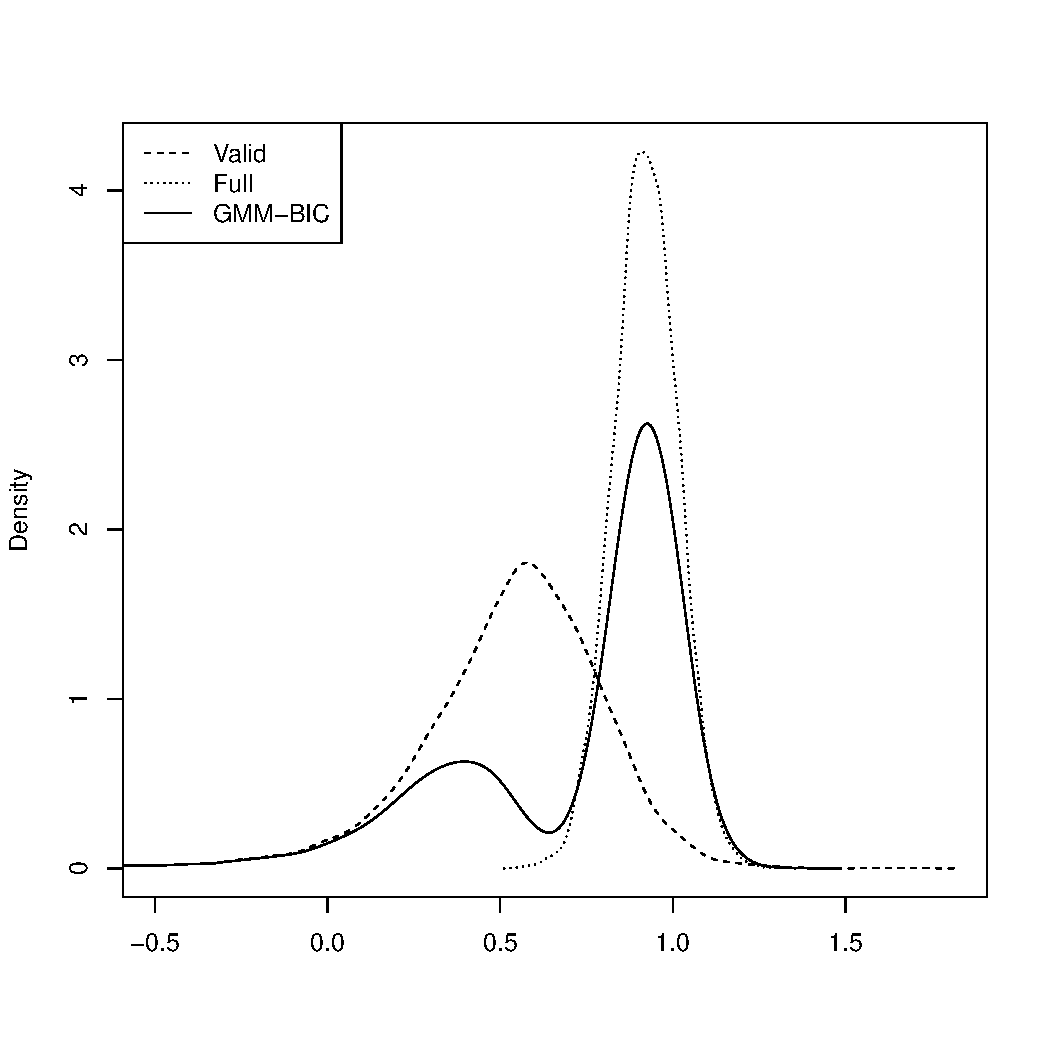
\includegraphics[scale = 0.48]{GMM_BIC}
	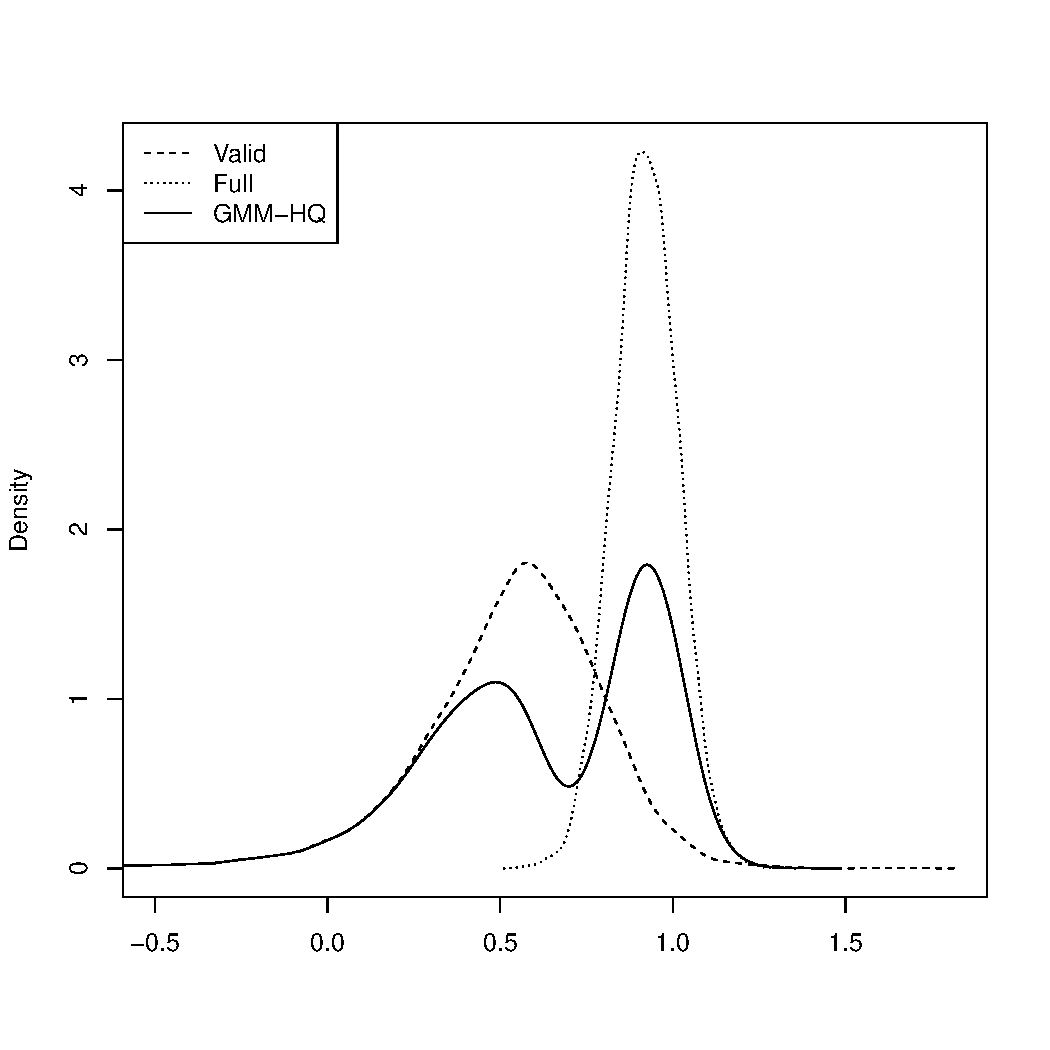
\includegraphics[scale = 0.48]{GMM_HQ}
\caption{ \small Post-selection distributions for the estimated effect of $x$ on $y$ in Equation \ref{eq:secondstage} with $\gamma = 0.4$, $\rho = 0.2$, $N=500$. The distribution post-GMM-BIC selection appears in the top panel, while the distribution post-GMM-HQ selection appears in the bottom panel. The distribution of the full estimator is given in dotted lines while that of the valid estimator is given in dashed lines in each panel. All distributions are calculated by kernel density estimation based on 10,000 simulation replications generated from Equations \ref{eq:secondstage}--\ref{eq:varmatrix}.}
\label{fig:consist}
\end{center}
\end{figure}
While Figure \ref{fig:consist} examines only one point in the parameter space the problem is more general, as shown by Table \ref{tab:BICcov}. 
The empirical coverage probabilities of traditional $95\%$ confidence intervals are far lower than their nominal level over the majority of the parameter space and the lack of uniformity is striking: small changes in parameters lead to large changes in coverage.

% latex.default(cover.BIC, file = outfilename, greek = TRUE, numeric.dollar = FALSE,      na.blank = TRUE, landscape = FALSE, rowname = NULL, append = TRUE) 
%
\begin{table}[!tbp]
\caption{Coverage post-GMM-BIC moment selection (nominal 95\%).}
\label{tab:BICcov}
\small
 \begin{center}
 \begin{tabular}{r|rrrrrrrrr}\hline\hline
&\multicolumn{9}{c}{$\rho = Cov(w,u)$}\\
\multicolumn{1}{c|}{$N = 500$}&\multicolumn{1}{c}{0}&\multicolumn{1}{c}{0.05}&\multicolumn{1}{c}{0.10}&\multicolumn{1}{c}{0.15}&\multicolumn{1}{c}{0.20}&\multicolumn{1}{c}{0.25}&\multicolumn{1}{c}{0.30}&\multicolumn{1}{c}{0.35}&\multicolumn{1}{c}{0.40}\tabularnewline
\hline
0.0&0.92&0.92&0.92&0.93&0.92&0.92&0.92&0.92&0.93\tabularnewline
0.1&0.92&0.83&0.77&0.83&0.90&0.92&0.93&0.92&0.92\tabularnewline
0.2&0.93&0.76&0.55&0.57&0.74&0.86&0.89&0.90&0.91\tabularnewline
0.3&0.93&0.75&0.45&0.35&0.50&0.69&0.80&0.85&0.88\tabularnewline
0.4&0.93&0.75&0.40&0.22&0.31&0.48&0.63&0.74&0.80\tabularnewline
0.5&0.93&0.75&0.38&0.18&0.20&0.32&0.46&0.59&0.68\tabularnewline
0.6&0.94&0.76&0.38&0.14&0.14&0.23&0.32&0.43&0.53\tabularnewline
\multirow{4}{5mm}{\begin{sideways}\parbox{1mm}{$\gamma\;$=$\;Cov(w,x)$}\end{sideways}}
0.7&0.94&0.76&0.37&0.12&0.11&0.16&0.24&0.32&0.42\tabularnewline
0.8&0.93&0.76&0.37&0.11&0.08&0.12&0.18&0.25&0.33\tabularnewline
0.9&0.94&0.75&0.37&0.11&0.07&0.10&0.14&0.19&0.25\tabularnewline
1.0&0.93&0.76&0.37&0.10&0.06&0.08&0.11&0.16&0.20\tabularnewline
1.1&0.93&0.77&0.37&0.10&0.06&0.07&0.10&0.13&0.16\tabularnewline
1.2&0.94&0.77&0.38&0.10&0.05&0.06&0.08&0.11&0.14\tabularnewline
1.3&0.94&0.77&0.38&0.10&0.04&0.05&0.07&0.09&0.12\tabularnewline
\hline
\end{tabular}
\end{center}
\footnotesize
\begin{tablenotes}
\item Values are calculated by simulating from Equations \ref{eq:secondstage}--\ref{eq:varmatrix} with $10,000$ replications.
\end{tablenotes}
\end{table}

In constrast to those of consistent selection, the asymptotics of \emph{conservative} selection  under local mis-specification provide a far more accurate picture of the distribution of post-selection estimators.
The point is \emph{not} that conservative criteria -- such as the FMSC, GMM-AIC and $J$-test at a fixed significance level -- are immune to the effects of selection on inference.
%The coverage probabilities for post-FMSC estimators given in Table \ref{tab:FMSCconf}, for example, show that this is not the case.
Rather, it is that conservative criteria can be studied in a framework that allows us to capture the non-normality that is so apparent from Figure \ref{fig:consist} in our limit theory.  
To this end, the present section derives the asymptotic distribution of generic ``moment average'' estimators by extending the idea behind the frequentist model average estimators of \cite{HjortClaeskens}. 
Such estimators are interesting in their own right and include, as a special case, a variety of post-conservative moment selection estimators including the FMSC.
Although their limit distributions are complicated, it remains possible to construct asymptotically valid confidence intervals for moment average estimators using a two-step, simulation-based procedure.
We begin by defining moment average estimators in general and considering some examples before presenting the procedure for constructing valid confidence intervals.

\subsection{Moment Average Estimators}
A generic moment average estimator takes the form
\begin{equation}
	\label{eq:avg}
	\widehat{\mu}=\sum_{S \in \mathscr{S}} \widehat{\omega}_S\widehat{\mu}_S
\end{equation}
where $\widehat{\mu}_S = \mu(\widehat{\theta}_S)$ is the estimator of the target parameter $\mu$ under moment set $S$, $\mathscr{S}$ is the collection of all moment sets under consideration, and $\widehat{\omega}_S$ is shorthand for the value of a data-dependent weight function  $\widehat{\omega}_S=\omega(\cdot, \cdot)$ evaluated at moment set $S$ and the sample observations $Z_{n1}, \hdots, Z_{nn}$.  
As above $\mu(\cdot)$ is a $\mathbb{R}$-valued, $Z$-almost surely continuous function of $\theta$ that is differentiable in an open neighborhood of $\theta_0$. When $\widehat{\omega}_S$ is an indicator, taking on the value one at the moment set moment set that minimizes some moment selection criterion, $\widehat{\mu}$ is a post-moment selection estimator. To characterize the limit distribution of $\widehat{\mu}$, we impose the following conditions on $\widehat{\omega}_S$.
\begin{assump}[Conditions on the Weights]\mbox{}
\label{assump:weights}
\begin{enumerate}[(a)]
	\item $\sum_{S \in \mathscr{S}} \widehat{\omega}_S = 1$, almost surely 
	\item For each $S\in \mathscr{S}$, $\widehat{\omega}_S \rightarrow_d\varphi_S(\tau, M)$, an almost-surely continuous function of $\tau$, $M$ and consistently estimable constants only.
\end{enumerate}
\end{assump}

\begin{cor}[Asymptotic Distribution of Moment-Average Estimators]
\label{cor:momentavg}
Under Assumption \ref{assump:weights} and the conditions of Theorem \ref{thm:normality},
	$$\sqrt{n}\left(\widehat{\mu} -  \mu_0\right) \rightarrow_{d}\Lambda(\tau) =  -\nabla_\theta\mu(\theta_0)'\left[\sum_{S \in \mathscr{S}} \varphi_S(\tau,M) K_S\Xi_S\right] \left(M + \left[\begin{array}
	{c} 0 \\ \tau
\end{array} \right]\right).$$
\end{cor}
Notice that the limit random variable from Corollary \ref{cor:momentavg}, denoted $\Lambda(\tau)$, is a \emph{randomly weighted average} of the multivariate normal vector $M$. 
Hence, $\Lambda(\tau)$ is non-normal. 
This is precisely the behavior that Figure \ref{fig:consist} suggests our limit theory should capture.
The conditions of Assumption \ref{assump:weights} are fairly mild. 
Requiring that the weights sum to one ensures that $\widehat{\mu}$ is a consistent estimator of $\mu_0$ and leads to a simpler expression for the limit distribution. 
While somewhat less transparent, the second condition is satisfied by weighting schemes based on a number of familiar moment selection criteria.
We see immediately from Corollary \ref{cor:FMSClimit}, for example, that the FMSC converges in distribution to a function of $\tau$, $M$ and consistently estimable constants only. 
The same ss true for the $J$-test statistic, as we see from the following result. 
\begin{thm}[Distribution of $J$-Statistic under Local Mis-Specification] 
\label{pro:jstat}
	Define the J-test statistic as per usual by $J_n(S)  = n \left[\Xi_S f_n(\widehat{\theta}_S)\right]' \widehat{\Omega}^{-1}\left[\Xi_S f_n(\widehat{\theta}_S)\right]$ where $\widehat{\Omega}^{-1}_S$ is a consistent estimator of $\Omega_S^{-1}$. Then, under the conditions of Theorem \ref{thm:normality}, we have $J_n(S) \rightarrow_dJ_S(\tau, M)$ where
		$$J_S(\tau, M)=[\Omega_S^{-1/2}(M_S + \tau_S)]' (I - P_S)[\Omega_S^{-1/2}\Xi_S(M_S + \tau_S)],$$
$M_S = \Xi_S M$, $\tau_S' = (0', \tau')\Xi_S'$, and $P_S$ is the projection matrix formed from the GMM identifying restrictions $\Omega^{-1/2}_S F_S$.
\end{thm}
Hence, normalized weights constructed from almost-surely continuous functions of either the FMSC or the $J$-test statistic satisfy Assumption \ref{assump:weights}. 

Post-selection estimators are merely a special cases of moment average estimators.
To see why, consider the weight function
$$\widehat{\omega}_S^{MSC} = \mathbf{1}\left\{\mbox{MSC}_n(S) = \min_{S'\in \mathscr{S}} \mbox{MSC}_n(S')\right\}$$where $\mbox{MSC}_n(S)$ is the value of some moment selection criterion evaluated at the sample observations $Z_{n1}\hdots, Z_{nn}$. 
Now suppose $\mbox{MSC}_n(S) \rightarrow_d\mbox{MSC}_S(\tau,M)$, a function of $\tau$, $M$ and consistently estimable constants only. 
Then, so long as the probability of ties, $P\left\{\mbox{MSC}_S(\tau,M) = \mbox{MSC}_{S'}(\tau,M) \right\}$, is zero for all $S\neq S'$, the continuous mapping theorem gives 
	$$\widehat{\omega}_S^{MSC} \rightarrow_d \mathbf{1}\left\{\mbox{MSC}_S(\tau,M) = \min_{S'\in \mathscr{S}} \mbox{MSC}_{S'}(\tau,M)\right\}$$ 
satisfying Assumption \ref{assump:weights} (b). 
Thus, post-selection estimators based on the FMSC, the downward $J$-test procedure, GMM-BIC, GMM-HQ, and GMM-AIC all fall within the ambit of \ref{cor:momentavg}. 
GMM-BIC and GMM-HQ, however, are not particularly interesting under local mis-specification.
Intuitively, because they aim to select all valid moment conditions w.p.a.1, we would expect that under Assumption \ref{assump:drift} they simply choose the full moment set in the limit. 
The following result states that this intuition is correct. 
\begin{thm}[Consistent Criteria under Local Mis-Specification]
\label{pro:andrews}
Consider a moment selection criterion of the form $MSC(S) = J_n(S) - h(|S|)\kappa_n$, where $h$ is strictly increasing,  $\lim_{n\rightarrow \infty}\kappa_n = \infty$, and $\kappa_n = o(n)$. Under the conditions of Theorem \ref{thm:normality}, $MSC(S)$ selects the full moment set with probability approaching one.
\end{thm}
The preceding result is a special case of a more general phenomenon: consistent selection procedures cannot detect model violations of order $O(n^{-1/2})$.
Because moment selection using the GMM-BIC or HQ leads to weights with a degenerate asymptotic distribution, one that does not capture the effects of selection on inference, these criteria are not considered further below. 

\subsection{Moment Averaging Examples}
Although it is a special case of moment averaging, moment selection is a somewhat crude procedure: it gives full weight to the estimator that minimizes the moment selection criterion no matter how close its nearest competitor lies. 
Accordingly, when competing moment sets have similar criterion values in the population, sampling variation can be \emph{magnified} in the selected estimator. 
Thus, it may be possible to achieve better performance by using smooth weights rather than discrete selection.
In this section we explore this possibility via two examples: one based on a simple heursitic and another on more detailed analytical calculations.

\subsubsection{Exponential Weights}
\todo[inline]{Possibly remove this section later.}
In the context of maximum likelihood estimation, \cite{Burnhametal} suggest averaging the estimators resulting from a number of competing models using exponential weights of the form $w_k = \exp(-I_k/2)/\sum_{i=1}^K \exp(-I_i/2)$ where $I_k$ is an information criterion evaluated for model $k$, and $i$ indexes the set of $K$ candidate models. This expression, constructed by an analogy with Bayesian model averaging, gives more weight to models with lower values of the information criterion but non-zero weight to all models. Applying this idea to the moment selection criteria given above, consider
	\begin{equation}	
		\widehat{\omega}_S = \left.\exp\left\{-\frac{\kappa}{2} \mbox{MSC}(S)\right\}\right/\sum_{S' \in \mathscr{S}}\exp\left\{-\frac{\kappa}{2} \mbox{MSC}(S')\right\}
		\label{eq:expweight}
\end{equation}
where MSC$(\cdot)$ is a moment selection criterion and the parameter $\kappa$ varies the uniformity of the weighting. As $\kappa \rightarrow 0$ the weights become more uniform; as $\kappa \rightarrow \infty$ they approach the moment selection procedure given by minimizing the corresponding criterion. Table \ref{tab:avg} compares moment averaging against moment selection by substituting FMSC, GMM-AIC, BIC and HQ into Equation \ref{eq:expweight} using the simulation experiment described in Section \ref{sec:fmscsim}. Calculations are based on 10,000 replications, each with a sample size of 500. For FMSC averaging $\kappa = 1/100$ to account for the fact that the FMSC is generally more variable than criteria based on the $J$-test. Weights for GMM-BIC, HQ, and AIC averaging set $\kappa = 1$. Both in terms of average and worst-case RMSE, moment selection is inferior to moment averaging. The only exception is worst-case RMSE for the FMSC. (Pointwise comparisons are available upon request.) If our goal is estimators with low RMSE, moment averaging may be preferable to moment selection. 


% latex.default(RMSE.average.vs.select, file = outfilename, greek = TRUE,      numeric.dollar = FALSE, na.blank = TRUE, landscape = FALSE,      append = TRUE) 
%
\begin{table}[!tbp]
 \begin{center}
\caption{Average and worst-case RMSE of moment averaging versus selection.}
\label{tab:avg}
\small
 \begin{tabular}{lrr}\hline\hline
\multicolumn{1}{l}{Average RMSE}&\multicolumn{1}{c}{Averaging}&\multicolumn{1}{c}{Selection}\tabularnewline
\hline
FMSC&0.24&0.26\tabularnewline
GMM-BIC&0.26&0.29\tabularnewline
GMM-HQ&0.26&0.29\tabularnewline
GMM-AIC&0.26&0.28\tabularnewline
\hline
\multicolumn{1}{l}{Worst-Case RMSE}&\multicolumn{1}{c}{Averaging}&\multicolumn{1}{c}{Selection}\tabularnewline
\hline
FMSC&0.36&0.33\tabularnewline
GMM-BIC&0.41&0.47\tabularnewline
GMM-HQ&0.36&0.39\tabularnewline
GMM-AIC&0.33&0.35\tabularnewline
\hline
\end{tabular}
\end{center}
\footnotesize
\begin{tablenotes}
	\item  Averaging is based on $\kappa = 1/100$ for FMSC weights and $\kappa = 1$ for all other weights. Values are calculated by simulating from Equations \ref{eq:secondstage}--\ref{eq:varmatrix} with $10,000$ replications at each combination of parameter values from Table \ref{tab:trueRMSE} and a sample size of $500$.
\end{tablenotes}
\end{table}

\subsubsection{Minimum AMSE Weights for OLS versus 2SLS Example}
The preceding example was based on the simple heuristic of ``exponential smoothing.'' 
In some applications, however, it is possible to \emph{analytically} derive weights that minimize AMSE.\footnote{I thank Bruce Hansen for suggesting this idea.} 
The OLS versus 2SLS example from Sections \ref{sec:OLSvsIVlowlevel} and \ref{sec:FMSCforOLSvsIV} is one such case. 

To begin, define an arbitrary weighted average of the OLS and 2SLS estimators from Equations \ref{eq:OLS} and \ref{eq:2SLS} by  
\begin{equation}
	\widetilde{\beta}(\omega) = \omega \widehat{\beta}_{OLS} + (1 - \omega) \widetilde{\beta}_{2SLS}
\end{equation}
where $\omega \in [0,1]$ is the weight given to the OLS estimator.
Since the weights sum to one, we have
\begin{eqnarray*}
	\sqrt{n}\left[\widehat{\beta}(\omega) - \beta \right] &=& \left[ \begin{array}
	{cc} \omega & (1 - \omega)
\end{array}\right] \left[
\begin{array}{c}
  \sqrt{n}(\widehat{\beta}_{OLS} - \beta) \\
  \sqrt{n}(\widetilde{\beta}_{2SLS} - \beta)
\end{array}
\right]\\
& \overset{d}{\rightarrow} & N\left(\mbox{Bias}\left[\widehat{\beta}(\omega)\right], Var\left[\widehat{\beta}(\omega)\right] \right)
\end{eqnarray*}
by Theorem \ref{thm:OLSvsIV}, where
\begin{eqnarray*}
	\mbox{Bias}\left[\widehat{\beta}(\omega)\right] &=& \omega \left( \frac{\tau}{\sigma_x^2} \right) \\
	 Var\left[\widehat{\beta}(\omega)\right] &=&  \frac{\sigma_\epsilon^2}{\sigma_x^2} \left[(2\omega^2 - \omega)\left( \frac{\sigma_x^2}{\gamma^2} - 1\right)+\frac{\sigma_x^2}{\gamma^2} \right]
\end{eqnarray*}
and accordingly
\begin{equation}
	\mbox{AMSE}\left[\widehat{\beta}(\omega) \right] =  \omega^2 \left(\frac{\tau^2}{\sigma_x^4} \right) + (\omega^2 - 2 \omega)\left(\frac{\sigma_\epsilon^2}{\sigma_x^2}\right)\left( \frac{\sigma_x^2}{\gamma^2} - 1\right) + \frac{\sigma_\epsilon^2}{\gamma^2}.
\end{equation}
The preceding is a globally convex function of $\omega$. 
Taking the first order condition and rearranging, we find that the unique global minimizer is
\begin{equation}
\label{eq:AMSEoptimal}
	\omega^* = \underset{\omega \in [0,1]}{\mbox{argmin}}\; \mbox{AMSE}\left[\widehat{\beta}(\omega) \right] 
	=\left[1 + \frac{\tau^2/\sigma_x^4}{\sigma_\epsilon^2(1/\gamma^2 - 1/\sigma_x^2)}\right]^{-1}
\end{equation}
In other words,
$$\omega^* = \left[1 + \frac{\mbox{ABIAS(OLS)}^2}{\mbox{AVAR(2SLS)}-\mbox{AVAR(OLS)}} \right]^{-1}$$

The preceding expression has several important consequences. 
First, since the variance of the 2SLS estimator is always strictly greater than that of the OLS estimator, the optimal value of $\omega$ \emph{cannot} be zero. 
No matter how strong the endogeneity of $x$ as measured by $\tau$, we should always give some weight to the OLS estimator. 
Second, when $\tau = 0$ the optimal value of $\omega$ is one. If $x$ is exogenous, OLS is strictly preferable to 2SLS. 
Third, the optimal weights depend on the strength of the instruments $\mathbf{z}$ as measured by $\gamma$. 
For a given value of $\tau\neq 0$, the stronger the instruments, the less weight we should give to OLS.

Equation \ref{eq:AMSEoptimal} gives the AMSE-optimal weighted average of the OLS and 2SLS estimators. 
To actually use the corresponding moment average estimator in practice, however, we need to estimate the unknowns.
As discussed above in Section \ref{sec:FMSCforOLSvsIV} the usual estimators of $\sigma_x^2$ and $\gamma$ remain consistent under local mis-specification, and the residuals from the 2SLS estimator provide a robust estimator of $\sigma_\epsilon^2$.
As before, the problem is estimating $\tau^2$.
A natural idea is to substitute the asymptotically unbiased estimator that arises from Theorem \ref{thm:tauOLSvsIV}, namely $\widehat{\tau}^2 - \widehat{V}$. 
The problem with this approach is that, while $\tau^2$ is always greater than or equal to zero as is $\widehat{\tau}^2$, the difference $\widehat{\tau}^2 - \widehat{V}$ \emph{can easily be negative}, yielding a \emph{negative} estimate of $\mbox{ABIAS(OLS)}^2$.
To solve this problem, we borrow an idea from the literature on shrinkage estimation and use the \emph{positive part} instead, namely $\max\left\{0, \; \widehat{\tau}^2 - \widehat{V}\right\}$, as in the positive-part James-Stein estimator.
This ensures that our estimator of $\omega^*$ lies inside the interval $[0,1]$.
Accordingly, we define 
\begin{equation}
	\widehat{\beta}^*_{AVG} = \widehat{\omega}^* \widehat{\beta}_{OLS} + (1 - \widehat{\omega}^*)\widetilde{\beta}_{2SLS}
\end{equation}
where
\begin{equation}
\widehat{\omega }^* = \left[1 + \frac{\max \left\{0, \; \left(\widehat{\tau}^2 - \widehat{\sigma}_\epsilon^2\widehat{\sigma}_x^2  \left(\widehat{\sigma}_x^2/\widehat{\gamma}^2 - 1 \right) \right)/\;\widehat{\sigma}_x^4 \right\}}{\widehat{\sigma}_\epsilon^2 (1/\widehat{\gamma}^2 - 1/\widehat{\sigma}_x^2)}\right]^{-1}
\end{equation}
 
\todo[inline]{Add simulation study. Also talk about how the estimator of the weight isn't asymptotically unbiased and how we might want to try other approaches, a question we leave for future research. This section is meant to illustrate the possibilities for moment averaging.
In the simulations, it works well. How to get a CI for such a procedure? We'll see in the next section.}

\subsection{Valid Confidence Intervals}
While Corollary \ref{cor:momentavg} characterizes the limiting behavior of moment-average, and hence post-selection estimators, the limiting random variable $\Lambda(\tau)$ is a complicated function of the normal random vector $M$. 
Because this distribution is analytically intractable, I adapt a suggestion from \cite{ClaeskensHjortbook} and approximate it by simulation.
The result is a conservative procedure that provides asymptotically valid confidence intervals for moment average and hence post-conservative selection estimators.\footnote{Although I originally developed this procedure by analogy to \cite{ClaeskensHjortbook}, \cite{Leeb} kindly pointed out that constructions of the kind given here have appeared elsewhere in the statistics literature, notably in \cite{Loh1985}, \cite{Berger1994}, and \cite{Silvapulle1996}. 
More recently, \cite{McCloskey} uses a similar approach to study non-standard testing problems.}
 
First, suppose that $K_S$, $\varphi_S$, $\theta_0$, $\Omega$ and $\tau$ were known. 
Then, by simulating from $M$, as defined in Theorem \ref{thm:normality}, the distribution of $\Lambda(\tau)$, defined in Corollary \ref{cor:momentavg}, could be approximated to arbitrary precision. 
To operationalize this procedure, substitute consistent estimators of $K_S$, $\theta_0$, and $\Omega$, e.g.\ those used to calculate FMSC. 
To estimate $\varphi_S$, we first need to derive the limit distribution of $\widehat{\omega}_S$, the data-based weights specified by the user. 
As an example, consider the case of moment selection based on the FMSC. Here $\widehat{\omega}_S$ is simply the indicator function
\begin{equation}
	\label{eq:FMSCindicate}
	\widehat{\omega}_S = \mathbf{1}\left\{\mbox{FMSC}_n(S) = \min_{S'\in \mathscr{S}} \mbox{FMSC}_n(S')\right\}
\end{equation}
To estimate $\varphi_S$, we first substitute consistent estimators of $\Omega$, $K_S$ and $\theta_0$ into $\mbox{FMSC}_S(\tau,M)$, defined in Corollary \ref{cor:FMSClimit}, yielding,
\begin{equation}
	\widehat{\mbox{FMSC}}_S(\tau,M) = \nabla_\theta\mu(\widehat{\theta})'\widehat{K}_S\Xi_S \left\{\left[\begin{array}{cc}0&0\\0&\widehat{\mathcal{B}}(\tau,M) \end{array}\right] + \widehat{\Omega}\right\}\Xi_S'\widehat{K}_S'\nabla_\theta\mu(\widehat{\theta}).
\end{equation}
where
\begin{equation}
	\widehat{\mathcal{B}}(\tau,M) = (\widehat{\Psi} M + \tau)(\widehat{\Psi} M + \tau)' - \widehat{\Psi} \widehat{\Omega} \widehat{\Psi}
\end{equation}
Combining this with Equation \ref{eq:FMSCindicate},
\begin{equation}
\label{eq:omegahat}
	\widehat{\varphi}_S(\tau,M) = \mathbf{1}\left\{\widehat{\mbox{FMSC}}_S(\tau,M) = \min_{S'\in \mathscr{S}} \widehat{\mbox{FMSC}}_{S'}(\tau,M)\right\}
\end{equation}
For GMM-AIC moment selection or selection based on a downward $J$-test, $\varphi_S(\cdot,\cdot)$ may be estimated analogously, following  Theorem \ref{pro:jstat}. 

Although simulating draws from $M$, defined in Theorem \ref{thm:normality}, requires only an estimate of $\Omega$, the limit $\varphi_S$ of the weight function also depends on $\tau$. 
As discussed above, no consistent estimator of $\tau$ is available under local mis-specification: the estimator $\widehat{\tau}$ has a non-degenerate limit distribution (see Theorem \ref{thm:tau}). 
Thus, substituting $\widehat{\tau}$ for $\tau$ will give erroneous results by failing to account for the uncertainty that enters through $\widehat{\tau}$. 
The solution is to use a two-stage procedure. 
First construct a  $100(1-\delta)\%$ confidence region $\mathscr{T}(\widehat{\tau},\delta)$ for $\tau$ using Theorem \ref{thm:tau}. 
Then, for each $\tau^* \in \mathscr{T}(\widehat{\tau},\delta)$ simulate from the distribution of $\Lambda(\tau^*)$, defined in Corollary \ref{cor:momentavg}, to obtain a \emph{collection} of $(1-\alpha)\times 100\%$ confidence intervals indexed by $\tau^*$. 
Taking the lower and upper bounds of these yields a \emph{conservative} confidence interval for $\widehat{\mu}$, as defined in defined in Equation \ref{eq:avg}. 
This interval has asymptotic coverage probability of \emph{at least} $(1-\alpha-\delta)\times 100\%$.
The precise algorithm is as follows.
\begin{alg}[Simulation-based Confidence Interval for $\widehat{\mu}$]
\label{alg:conf}
\mbox{}
\begin{enumerate}
	\item For each $\tau^* \in \mathscr{T}(\widehat{\tau},\delta)$ 
		\begin{enumerate}[(i)]
			\item Generate $J$ independent draws $M_j \sim N_{p+q}( 0, \widehat{\Omega} )$
			\item Set $\Lambda_j(\tau^*) = -\nabla_\theta\mu(\widehat{\theta})'\left[\sum_{S \in \mathscr{S}} \widehat{\varphi}_S(\tau^*,M_j) \widehat{K}_S\Xi_S\right] (M_j + \tau^*)$
			\item Using the draws $\{\Lambda_j(\tau^*)\}_{j=1}^J$, calculate $\widehat{a}(\tau^*)$, $\widehat{b}(\tau^*)$ such that
		$$P\left\{ \widehat{a}(\tau^*) \leq\Lambda(\tau^*)\leq \widehat{b}(\tau^*) \right\} = 1 - \alpha$$
		\end{enumerate}
	\item Set $\displaystyle \widehat{a}_{min}(\widehat{\tau})=\min_{\tau^* \in \mathscr{T}(\widehat{\tau},\delta)} \widehat{a}(\tau^*)$ and $\displaystyle \widehat{b}_{max}(\widehat{\tau})= \max_{\tau^* \in \mathscr{T}(\widehat{\tau},\delta)} \widehat{b}(\tau^*)$ \vspace{0.5em}
	\item The confidence interval for $\mu$ is
				$\displaystyle \mbox{CI}_{sim}=\left[ \widehat{\mu} - \frac{\widehat{b}_{max}(\widehat{\tau})}{\sqrt{n}}, \;\;\; \widehat{\mu} - \frac{\widehat{a}_{min}(\widehat{\tau})}{\sqrt{n}} \right]$
\end{enumerate}
\end{alg}

\begin{thm}[Simulation-based Confidence Interval for $\widehat{\mu}$]
\label{pro:sim}
Let $\widehat{\Psi}$, $\widehat{\Omega}$, $\widehat{\theta}$, $\widehat{K}_S$, $\widehat{\varphi}_S$ be consistent estimators of $\Psi$, $\Omega$, $\theta_0$, $K_S$, $\varphi_S$ and define 
\begin{eqnarray*}
	\Delta_n(\widehat{\tau},\tau^*) &=& \left(\widehat{\tau} - \tau^*\right)' \left(\widehat{\Psi}\widehat{\Omega}\widehat{\Psi}'\right)^{-1} \left(\widehat{\tau} - \tau^*\right)\\
	\mathscr{T}(\widehat{\tau},\delta) &=& \left\{\tau^* \colon  \Delta_n(\widehat{\tau},\tau^*) \leq \chi^2_q(\delta)\right\}
\end{eqnarray*}
where $\chi^2_q(\delta)$ denotes the $1-\delta$ quantile of a $\chi^2$ distribution with $q$ degrees of freedom.
Then, the interval $\mbox{CI}_{sim}$ defined in Algorithm \ref{alg:conf} has asymptotic coverage probability no less than $1-(\alpha + \delta)$ as $J,n\rightarrow \infty$.
\end{thm}

\todo[inline]{Need to talk about coverage versus width. Explore in the simulations and empirical example. There is a cost to moment selection. But this cost is still present when selection is carried out informally: we're just trying to make it formal here. Also talk about how we could use the same procedure to get an interval for more general moment average estimators.}

To evaluate the performance of the procedure given in Algorithm \ref{alg:conf}, we revisit the simulation experiment described in Section \ref{sec:fmscsim}, considering FMSC moment selection. The following results are based on 10,000 replications, each with a sample size of 500. Table \ref{tab:FMSCconf} gives the empirical coverage probabilities of traditional 95\% confidence intervals post-FMSC selection. These are far below the nominal level over the vast majority of the parameter space. Table \ref{tab:FMSCcorrect} presents the empirical coverage of conservative 90\% confidence intervals constructed according to Algorithm \ref{alg:conf}, with $B=1000$.\footnote{Because this simulation is computationally intensive, I use a reduced grid of parameter values.} The two-stage simulation procedure performs remarkably well, achieving a minimum coverage probability of $0.89$ relative to its nominal level of $0.9$. Moreover, a na\"{i}ve one-step procedure that omits the first-stage and simply simulates from $M$ based on $\widehat{\tau}$ performs surprisingly well; see Table \ref{tab:FMSCnaive}. While the empirical coverage probabilities of the one-step procedure are generally lower than the nominal level of $0.95$, they represent a substantial improvement over the traditional intervals given in Table \ref{tab:FMSCconf}, with a worst-case coverage of $0.72$ compared to $0.15$. This suggests that the one-step intervals might be used as a rough but useful approximation to the correct but more computationally intensive intervals constructed according to Algorithm \ref{alg:conf}.

% latex.default(cover.FMSC, file = outfilename, greek = TRUE, numeric.dollar = FALSE,      na.blank = TRUE, landscape = FALSE, rowname = NULL, append = TRUE) 
%
\begin{table}[!tbp]
 \begin{center}
 \caption{Coverage post-FMSC moment selection (nominal 95\%).}
\label{tab:FMSCconf}
\small
 \begin{tabular}{r|rrrrrrrrr}\hline\hline
&\multicolumn{9}{c}{$\rho = Cov(w,u)$}\\
\multicolumn{1}{c|}{$N=500$}&\multicolumn{1}{c}{0}&\multicolumn{1}{c}{0.05}&\multicolumn{1}{c}{0.10}&\multicolumn{1}{c}{0.15}&\multicolumn{1}{c}{0.20}&\multicolumn{1}{c}{0.25}&\multicolumn{1}{c}{0.30}&\multicolumn{1}{c}{0.35}&\multicolumn{1}{c}{0.40}\tabularnewline
\hline
0.0&0.92&0.93&0.93&0.93&0.93&0.93&0.93&0.93&0.93\tabularnewline
0.1&0.91&0.87&0.88&0.91&0.93&0.93&0.93&0.93&0.93\tabularnewline
0.2&0.90&0.79&0.72&0.82&0.90&0.93&0.92&0.93&0.93\tabularnewline
0.3&0.90&0.76&0.58&0.64&0.80&0.90&0.92&0.93&0.93\tabularnewline
0.4&0.89&0.75&0.50&0.47&0.64&0.80&0.88&0.91&0.92\tabularnewline
0.5&0.89&0.74&0.45&0.36&0.50&0.67&0.79&0.87&0.91\tabularnewline
0.6&0.89&0.74&0.43&0.30&0.38&0.54&0.68&0.78&0.85\tabularnewline
\multirow{4}{5mm}{\begin{sideways}\parbox{1mm}{$\gamma\;$=$\;Cov(w,x)$}\end{sideways}}
0.7&0.90&0.74&0.41&0.24&0.31&0.44&0.57&0.68&0.78\tabularnewline
0.8&0.89&0.74&0.41&0.22&0.25&0.36&0.48&0.59&0.70\tabularnewline
0.9&0.91&0.74&0.41&0.20&0.21&0.31&0.41&0.52&0.61\tabularnewline
1.0&0.90&0.75&0.40&0.18&0.19&0.25&0.35&0.45&0.53\tabularnewline
1.1&0.90&0.76&0.40&0.17&0.17&0.23&0.32&0.39&0.47\tabularnewline
1.2&0.91&0.76&0.41&0.17&0.15&0.20&0.27&0.34&0.42\tabularnewline
1.3&0.92&0.77&0.41&0.16&0.15&0.19&0.24&0.31&0.39\tabularnewline
\hline
\end{tabular}
\end{center}
\footnotesize
\begin{tablenotes}
\item Values are calculated by simulating from Equations \ref{eq:secondstage}--\ref{eq:varmatrix} with $10,000$ replications.
\end{tablenotes}
\end{table}



% latex.default(conf.refined, file = outfilename, greek = TRUE,      numeric.dollar = FALSE, na.blank = TRUE, landscape = FALSE,      rowname = NULL, append = FALSE) 
%
\begin{table}[!tbp]
 \begin{center}
\caption{Coverage of conservative two-step interval post-FMSC (nominal >90\%)}
\label{tab:FMSCcorrect}
\small
 \begin{tabular}{r|rrrrr}\hline\hline
&\multicolumn{5}{c}{$\rho = Cov(w,u)$}\\
\multicolumn{1}{c|}{$N=500$}&\multicolumn{1}{c}{0}&\multicolumn{1}{c}{0.1}&\multicolumn{1}{c}{0.2}&\multicolumn{1}{c}{0.3}&\multicolumn{1}{c}{0.4}\tabularnewline
\hline
0.0&0.92&0.93&0.93&0.93&0.94\tabularnewline
0.2&0.95&0.91&0.93&0.95&0.97\tabularnewline
0.4&0.95&0.95&0.90&0.93&0.97\tabularnewline
0.6&0.95&0.95&0.92&0.90&0.92\tabularnewline
\multirow{4}{5mm}{\begin{sideways}\parbox{1mm}{$\gamma\;$=$\;Cov(w,x)$}\end{sideways}}
0.8&0.94&0.95&0.96&0.90&0.89\tabularnewline
1.0&0.94&0.94&0.96&0.93&0.90\tabularnewline
1.2&0.94&0.94&0.96&0.95&0.92\tabularnewline
\hline
\end{tabular}
\end{center}
\footnotesize
\begin{tablenotes}
	\item Intervals are calculated using Algorithm \ref{alg:conf} with $B = 1000$. Simulations are generated from Equations \ref{eq:secondstage}--\ref{eq:varmatrix} with $10,000$ replications.
\end{tablenotes}
\end{table}


% latex.default(conf.naive, file = outfilename, greek = TRUE, numeric.dollar = FALSE,      na.blank = TRUE, landscape = FALSE, rowname = NULL, append = FALSE) 
%
\begin{table}[!tbp]
\caption{Coverage of na\"{i}ve one-step interval post-FMSC (nominal 95\%)}
\label{tab:FMSCnaive}
\small
 \begin{center}
 \begin{tabular}{r|rrrrrrrrr}\hline\hline
&\multicolumn{9}{c}{$\rho = Cov(w,u)$}\\
\multicolumn{1}{c|}{$N=500$}&\multicolumn{1}{c}{0}&\multicolumn{1}{c}{0.05}&\multicolumn{1}{c}{0.10}&\multicolumn{1}{c}{0.15}&\multicolumn{1}{c}{0.20}&\multicolumn{1}{c}{0.25}&\multicolumn{1}{c}{0.30}&\multicolumn{1}{c}{0.35}&\multicolumn{1}{c}{0.40}\tabularnewline
\hline
0.0&0.93&0.92&0.93&0.93&0.93&0.93&0.93&0.93&0.94\tabularnewline
0.1&0.93&0.91&0.91&0.92&0.92&0.92&0.93&0.94&0.95\tabularnewline
0.2&0.94&0.91&0.86&0.87&0.92&0.93&0.94&0.95&0.96\tabularnewline
0.3&0.95&0.94&0.87&0.81&0.85&0.91&0.94&0.96&0.96\tabularnewline
0.4&0.95&0.95&0.91&0.82&0.77&0.84&0.90&0.94&0.95\tabularnewline
0.5&0.95&0.95&0.93&0.86&0.76&0.76&0.82&0.88&0.92\tabularnewline
0.6&0.94&0.94&0.94&0.90&0.80&0.74&0.75&0.81&0.87\tabularnewline
\multirow{4}{5mm}{\begin{sideways}\parbox{1mm}{$\gamma\;$=$\;Cov(w,x)$}\end{sideways}}
0.7&0.94&0.94&0.95&0.93&0.85&0.74&0.73&0.75&0.81\tabularnewline
0.8&0.94&0.94&0.95&0.94&0.88&0.79&0.73&0.73&0.76\tabularnewline
0.9&0.95&0.94&0.94&0.94&0.91&0.83&0.76&0.72&0.73\tabularnewline
1.0&0.95&0.94&0.94&0.94&0.92&0.86&0.78&0.73&0.73\tabularnewline
1.1&0.95&0.94&0.94&0.95&0.94&0.89&0.81&0.76&0.73\tabularnewline
1.2&0.95&0.94&0.94&0.95&0.94&0.90&0.85&0.79&0.75\tabularnewline
1.3&0.95&0.94&0.94&0.95&0.95&0.92&0.87&0.81&0.78\tabularnewline
\hline
\end{tabular}
\end{center}
\footnotesize
	\begin{tablenotes}
		\item Intervals are calculated by simulation with $B=1000$ using $\widehat{\tau}$ rather than constructing a confidence interval for $\tau$ (c.f.\ Algorithm \ref{alg:conf}). Simulations are generated from Equations \ref{eq:secondstage}--\ref{eq:varmatrix} with $10,000$ replications.
	\end{tablenotes}
\end{table}





\section{Empirical Example: Geography or Institutions?}
\label{sec:application}
\cite{Carstensen2006} address a controversial question from the development literature: does geography directly effect income after controlling for institutions? A number of well-known studies find little or no direct effect of geographic endowments. \cite{Acemoglu}, for example, find that countries nearer to the equator do not have lower incomes after controlling for institutions. \cite{Rodrik} report that geographic variables have only small direct effects on income, affecting development mainly through their influence on institutions. Similarly, \cite{Easterly} find no effect of ``tropics, germs and crops'' except through institutions. \cite{Sachs} responds directly to these three papers by showing that malaria transmission, a variable largely driven by ecological conditions, directly influences the level of per capita income, even after controlling for institutions. Because malaria transmission  is very likely endogenous, Sachs uses a measure of ``malaria ecology,'' constructed to be exogenous both to present economic conditions and public health interventions, as an instrument. \cite{Carstensen2006} address the robustness of Sachs's results using the following baseline regression for a sample of 45 countries:
\begin{equation}
	\mbox{ln\emph{gdpc}}_i = \beta_1 + \beta_2 \cdot \mbox{\emph{institutions}}_i + \beta_3 \cdot \mbox{\emph{malaria}}_i + \epsilon_i
\end{equation}
Treating both institutions and malaria transmission as endogenous, they consider a variety of measures of each and a number of instrument sets. In each case, they find large negative effects of malaria transmission, lending further support to Sach's conclusion. In this section, I expand on the instrument selection exercise given in Table 2 of \cite{Carstensen2006} using the FMSC and corrected confidence intervals described above. I consider two questions. First, based on the FMSC methodology, which instruments should we choose to produce the best estimate of $\beta_3$, the effect of malaria transmission on per capita income? Second, after correcting confidence intervals for instrument selection, do we still find evidence of large and negative effects of malaria transmission on income? All results given here are calculated by 2SLS using the formulas from Section \ref{sec:2sls} and the variables described in Table \ref{tab:desc}. In keeping with Table 2 of \cite{Carstensen2006}, I use ln\emph{gdpc} as the dependent variable and \emph{rule} and \emph{malfal} as measures of institutions and malaria transmission throughout. 


\begin{table}[!tbp]
\caption{Description of Variables}
\small
\label{tab:desc}
\begin{center}
\begin{tabular}{lll}
\hline \hline
Name& Description &\\
\hline
ln\emph{gdpc}&Real GDP/capita at PPP, 1995 International Dollars &Outcome\\
\emph{rule}&Institutional quality (Average Governance Indicator)&Regressor\\
\emph{malfal}&Fraction of population at risk of malaria transmission, 1994&Regressor\\
ln\emph{mort}&Log settler mortality (per 1000 settlers), early 19th century&Baseline\\
\emph{maleco}&Index of stability of malaria transmission&Baseline\\
\emph{frost}&Prop.\ of land receiving at least 5 days of frost in winter&Climate\\
\emph{humid}&Highest temp. in month with highest avg.\ afternoon humidity&Climate\\
\emph{latitude}&Distance from equator (absolute value of latitude in degrees)&Climate \\
\emph{eurfrac}&Fraction of pop.\ that speaks major West.\ European Language&Europe \\
\emph{engfrac}&Fraction of pop.\ that speaks English&Europe\\
\emph{coast}&Proportion of land area within 100km of sea coast&Openness\\
\emph{trade}&Log Frankel-Romer predicted trade share&Openness\\
\hline
\end{tabular}
\end{center}
\end{table}

To apply the FMSC to the present example, we need a minimum of two valid instruments besides the constant term. Based on the arguments given in \cite{Acemoglu}, \cite{Carstensen2006} and \cite{Sachs}, I proceed under the assumption that ln\emph{mort} and \emph{maleco}, measures of early settler mortality and malaria ecology, are exogenous. Rather than selecting over every possible subset of instruments, I consider a number of instrument blocks defined in \cite{Carstensen2006}. The baseline block contains ln\emph{mort}, \emph{maleco} and a constant; the climate block contains \emph{frost}, \emph{humid}, and \emph{latitude}; the Europe block contains \emph{eurfrac} and \emph{engfrac}; and the openness block contains \emph{coast} and \emph{trade}. Full descriptions of these variables appear in Table \ref{tab:desc}. Table \ref{tab:fullresults} gives 2SLS results and traditional 95\% confidence intervals for all instrument sets considered here.

% latex.default(Part1, file = "Output_Tables.tex", greek = TRUE,      numeric.dollar = FALSE, na.blank = TRUE, landscape = FALSE,      append = FALSE) 
%
\begin{sidewaystable}[!tbp]
\caption{2SLS Results for all Instrument Sets}
\label{tab:fullresults}
 \begin{center}
 \begin{tabular}{lrrrrrrrrrrrr}\hline\hline
&\multicolumn{2}{c}{1}&
\multicolumn{2}{c}{2}&
\multicolumn{2}{c}{3}&
\multicolumn{2}{c}{4}&
\multicolumn{2}{c}{5}&
\multicolumn{2}{c}{6}\tabularnewline
&\multicolumn{1}{c}{\emph{rule}}&\multicolumn{1}{c}{\emph{malfal}}&
\multicolumn{1}{c}{\emph{rule}}&\multicolumn{1}{c}{\emph{malfal}}&
\multicolumn{1}{c}{\emph{rule}}&\multicolumn{1}{c}{\emph{malfal}}&
\multicolumn{1}{c}{\emph{rule}}&\multicolumn{1}{c}{\emph{malfal}}&
\multicolumn{1}{c}{\emph{rule}}&\multicolumn{1}{c}{\emph{malfal}}&
\multicolumn{1}{c}{\emph{rule}}&\multicolumn{1}{c}{\emph{malfal}}\tabularnewline
\hline
coeff.&0.89&-1.04&0.97&-0.90&0.81&-1.09&0.86&-1.14&0.93&-1.02&0.86&-0.98\tabularnewline
SE&0.18& 0.30&0.16& 0.29&0.16& 0.29&0.16& 0.27&0.15& 0.26&0.14& 0.27\tabularnewline
lower&0.53&-1.65&0.65&-1.48&0.49&-1.67&0.55&-1.69&0.63&-1.54&0.59&-1.53\tabularnewline
upper&1.25&-0.43&1.30&-0.32&1.13&-0.51&1.18&-0.59&1.22&-0.49&1.14&-0.43\tabularnewline
&\multicolumn{2}{c}{Baseline}&\multicolumn{2}{c}{Baseline}&\multicolumn{2}{c}{Baseline}&\multicolumn{2}{c}{Baseline}&\multicolumn{2}{c}{Baseline}&\multicolumn{2}{c}{Baseline}\tabularnewline
&&&\multicolumn{2}{c}{Climate}&&&&&\multicolumn{2}{c}{Climate}&\multicolumn{2}{c}{Climate}\tabularnewline
&&&&&\multicolumn{2}{c}{Openness}&&&&&\multicolumn{2}{c}{Openness}\tabularnewline
&&&&&&&\multicolumn{2}{c}{Europe}&\multicolumn{2}{c}{Europe}&&\tabularnewline
\hline
\\ \\
\hline\hline
&\multicolumn{2}{c}{7}&
\multicolumn{2}{c}{8}&
\multicolumn{2}{c}{9}&
\multicolumn{2}{c}{10}&
\multicolumn{2}{c}{11}&
\multicolumn{2}{c}{12}\tabularnewline
&\multicolumn{1}{c}{\emph{rule}}&\multicolumn{1}{c}{\emph{malfal}}&
\multicolumn{1}{c}{\emph{rule}}&\multicolumn{1}{c}{\emph{malfal}}&
\multicolumn{1}{c}{\emph{rule}}&\multicolumn{1}{c}{\emph{malfal}}&
\multicolumn{1}{c}{\emph{rule}}&\multicolumn{1}{c}{\emph{malfal}}&
\multicolumn{1}{c}{\emph{rule}}&\multicolumn{1}{c}{\emph{malfal}}&
\multicolumn{1}{c}{\emph{rule}}&\multicolumn{1}{c}{\emph{malfal}}\tabularnewline
\hline
coeff.&0.81&-1.16&0.84&-1.08&0.93&-0.93&1.02&-0.85&1.02&-0.86&0.88&-1.00\tabularnewline
SE&0.15& 0.27&0.13& 0.25&0.16& 0.23&0.15& 0.27&0.15& 0.23&0.12& 0.21\tabularnewline
lower&0.51&-1.70&0.57&-1.58&0.61&-1.39&0.71&-1.39&0.72&-1.32&0.63&-1.42\tabularnewline
upper&1.11&-0.62&1.10&-0.58&1.26&-0.46&1.33&-0.30&1.32&-0.40&1.12&-0.57\tabularnewline
&\multicolumn{2}{c}{Baseline}&\multicolumn{2}{c}{Baseline}&\multicolumn{2}{c}{Baseline}&\multicolumn{2}{c}{Baseline}&\multicolumn{2}{c}{Baseline}&\multicolumn{2}{c}{Baseline}\tabularnewline
&&&\multicolumn{2}{c}{Climate}&&&&&&&\multicolumn{2}{c}{Climate}\tabularnewline
&\multicolumn{2}{c}{Openness}&\multicolumn{2}{c}{Openness}&& &&&&&\multicolumn{2}{c}{Openness}\tabularnewline
&\multicolumn{2}{c}{Europe}&\multicolumn{2}{c}{Europe}&& &&&&&\multicolumn{2}{c}{Europe}\tabularnewline
&&&&&\multicolumn{2}{c}{\emph{malfal}$^2$}&& &\multicolumn{2}{c}{\emph{malfal}$^2$}&\multicolumn{2}{c}{\emph{malfal}$^2$}\tabularnewline
&&&&&&&\multicolumn{2}{c}{\emph{rule}$^2$}&\multicolumn{2}{c}{\emph{rule}$^2$}&\multicolumn{2}{c}{\emph{rule}$^2$}\tabularnewline
\hline
\end{tabular}

\end{center}

\end{sidewaystable}


Table \ref{tab:replicate} presents FMSC results for instrument sets 1--8  as defined in Table \ref{tab:fullresults}. Results are presented for two cases: the first takes the effect of \emph{malfal}, a measure of malaria transmission, as the target parameter while the second uses the effect of \emph{rule}, a measure of institutions. In each case, the FMSC selects instrument set 8: the full instrument set containing the baseline, climate, Europe and openness blocks. The rankings, however, differ depending on the target parameter.  When the target is \emph{rule} instrument sets 8 and 5 are virtually identical in terms of FMSC: 0.26 versus 0.23. In Table 2 of their paper, \cite{Carstensen2006} report GMM-BIC and HQ results for selection over instrument sets 2--4 and 8 that also favor instrument set 8. However, the authors do not consider instrument sets 5--7. Although the FMSC also selects instrument set 8, the FMSC values of instrument set 5 are small enough to suggest that including the openness block does little to reduce MSE.

The bottom panel of Table \ref{tab:replicate} presents a number of alternative 95\% confidence intervals for the effects of \emph{malfal} and \emph{rule}, respectively. The first row gives the traditional asymptotic confidence interval from Table \ref{tab:fullresults}, while the following three give simulation-based intervals accounting for the effects of instrument selection. I do not present intervals for the conservative procedure given in Algorithm \ref{alg:conf} because the results in this example are so insensitive to the value of $\tau$ that the minimization and maximization problems given in Step 2 of the Algorithm are badly behaved. To illustrate this, I instead present intervals that use the same simulation procedure as Algorithm \ref{alg:conf} but treat $\tau$ as fixed. I consider four possible values of the bias parameter. When $\tau = \widehat{\tau}$, we have the one-step corrected interval considered in Table \ref{tab:FMSCnaive}. When $\tau = 0$, we have an interval that assumes all instruments are valid. The remaining two values $\widehat{\tau}_{min}$ and $\widehat{\tau}_{max}$ correspond to the lower and upper bounds of \emph{elementwise} 95\% confidence intervals for $\tau$ based on the distributional result given in Theorem \ref{thm:tau}. These result in a region with greater than 95\% coverage for $\tau$ considered jointly. Corrected 95\% intervals for the effect of \emph{malfal} are similar regardless of the value of $\tau$ used in the simulation, and the same is true for \emph{rule}. We find no evidence that accounting for the effects of instrument selection changes our conclusions about the sign or significance of \emph{malfal} or \emph{rule}.

\begin{table}[htbp]
\caption{FMSC values and confidence intervals for instrument sets 1--8.}
\label{tab:replicate}
\small
 \begin{center}
 \begin{tabular}{lcccc}\hline\hline
 & \multicolumn{2}{c}{$\mu=$\emph{malfal}}& \multicolumn{2}{c}{$\mu=$\emph{rule}}\\
&\multicolumn{1}{c}{FMSC}&\multicolumn{1}{c}{$\widehat{\mu}$}&\multicolumn{1}{c}{FMSC}&\multicolumn{1}{c}{$\widehat{\mu}$}\tabularnewline
\hline
Valid (1)&3.03&-1.04&1.27&0.89\tabularnewline
Climate (2)&2.67&-0.90&0.92&0.97\tabularnewline   
Openness (3)&2.31&-1.09&1.23&0.81\tabularnewline  
Europe (4)&1.83&-1.14&0.55&0.86\tabularnewline
Openness, Europe (7)&1.72&-1.16&0.77&0.81\tabularnewline  
Climate, Openness (6)&1.65&-0.98&0.43&0.86\tabularnewline
Climate, Europe (5)&0.71&-1.02&0.26&0.93\tabularnewline
Full (8)&0.53&-1.08&0.23&0.84\tabularnewline
\hline 
Traditional&\multicolumn{2}{c}{(-1.58, -0.58)}&\multicolumn{2}{c}{(0.57, 1.10)}\\
$\tau = \widehat{\tau}$&\multicolumn{2}{c}{(-1.54, -0.61)}&\multicolumn{2}{c}{(0.55, 1.13)}\\
$\tau = 0$&\multicolumn{2}{c}{(-1.53, -0.64)}&\multicolumn{2}{c}{(0.55, 1.12)}\\
$\tau = \widehat{\tau}_{max}$&\multicolumn{2}{c}{(-1.51, -0.55)}&\multicolumn{2}{c}{(0.55, 1.17)}\\
$\tau = \widehat{\tau}_{min}$&\multicolumn{2}{c}{(-1.61, -0.58)}&\multicolumn{2}{c}{(0.49, 1.15)}\\
\hline

\end{tabular}
\end{center}
\end{table}



FMSC is designed to include invalid instruments when doing so will reduce AMSE. Table \ref{tab:endog} considers adding two almost certainly invalid instruments to the baseline instrument set: \emph{rule}$^2$ and \emph{malfal}$^2$. Because they are constructed from the endogenous regressors, these instruments are likely to be highly relevant. Unless the effect of institutions and malaria transmission on GDP per capita is exactly linear, however, they are invalid. When the target is \emph{malfal}, we see that the FMSC selects an instrument set including \emph{malfal}$^2$ and the baseline instruments. FMSC is negative in this case. Although it provides an asymptotically unbiased estimator of AMSE, the FMSC may be negative because it subtracts $\widehat{\Psi}\widehat{\Omega}\widehat{\Psi}'$ from $\widehat{\tau}\widehat{\tau}'$ to estimate squared bias. When the target is \emph{rule}, FMSC chooses the full instrument set, including the baseline instruments along with \emph{rule}$^2$ and \emph{malfal}$^2$. While these instruments are likely invalid, FMSC chooses to include them because its estimate of the bias they induce is small compared to the reduction in variance they provide. Table \ref{tab:all} further expands the instrument sets under consideration to include 1--4 and 9--12. In this case, the FMSC chooses instrument set 12 for both target parameters. However, we see from the FMSC rankings that most of the reduction in MSE achieved by instrument set 12 comes from the inclusion of the squared endogenous regressors in the instrument set. Turning our attention to the confidence intervals in Tables \ref{tab:endog} and \ref{tab:all}, we again see that the simulation-based intervals are extremely insensitive to the value of $\tau$ used. Again, the sign and significance of \emph{malfal} and \emph{rule} is insensitive to the effects of instrument selection. These results lend support to the view of \cite{Carstensen2006} and \cite{Sachs} that malaria transmission has a direct effect on development.

\begin{table}[htbp]
\caption{FMSC values and confidence intervals for instrument sets 1 and 9--11}
\label{tab:endog}
\small
\centering
 \begin{tabular}{lrrrr}\hline\hline
 & \multicolumn{2}{c}{$\mu=$\emph{malfal}}& \multicolumn{2}{c}{$\mu=$\emph{rule}}\\
&\multicolumn{1}{c}{FMSC}&\multicolumn{1}{c}{$\widehat{\mu}$}&\multicolumn{1}{c}{FMSC}&\multicolumn{1}{c}{$\widehat{\mu}$}\tabularnewline
\hline
Valid (1)& 3.03&-1.04& 1.27&0.89\tabularnewline
\emph{rule}$^2$ (10)& 2.05&-0.84& 0.28&1.02\tabularnewline
Full (11)&-0.20&-0.85& -0.06&1.02\tabularnewline
\emph{malfal}$^2$ (9)&-0.41&-0.92&0.18&0.93\tabularnewline
\hline
Traditional&\multicolumn{2}{r}{(-1.39, -0.46)}&\multicolumn{2}{r}{(0.72, 1.32)}\\
$\tau = \widehat{\tau}$&\multicolumn{2}{r}{(-1.49, -0.38)}&\multicolumn{2}{r}{(0.68, 1.36)}\\
$\tau = 0$&\multicolumn{2}{r}{(-1.46, -0.38)}&\multicolumn{2}{r}{(0.71, 1.32)}\\
$\tau = \widehat{\tau}_{max}$&\multicolumn{2}{r}{(-1.51, -0.38)}&\multicolumn{2}{r}{(0.66, 1.37)}\\
$\tau = \widehat{\tau}_{min}$&\multicolumn{2}{r}{(-1.49, -0.38)}&\multicolumn{2}{r}{(0.71, 1.35)}\\
\hline
\end{tabular}


\footnotesize
\end{table}






\begin{table}[htbp]
\caption{FMSC values and confidence intervals for instrument sets 1--4 and 9--12}
\label{tab:all}
\small
\centering
 \begin{tabular}{lcccc}\hline\hline
 & \multicolumn{2}{c}{$\mu=$\emph{malfal}}& \multicolumn{2}{c}{$\mu=$\emph{rule}}\\
&\multicolumn{1}{c}{FMSC}&\multicolumn{1}{c}{$\widehat{\mu}$}&\multicolumn{1}{c}{FMSC}&\multicolumn{1}{c}{$\widehat{\mu}$}\tabularnewline
\hline
Valid (1)& 3.03&-1.04& 1.27&0.89\tabularnewline
Climate (2)& 2.85&-0.90& 0.95&0.97\tabularnewline
Openness (3)& 2.51&-1.09& 1.26&0.81\tabularnewline
Europe (4)& 1.94&-1.14& 0.58&0.86\tabularnewline
\emph{rule}$^2$ (10)& 1.88&-0.84& 0.25&1.02\tabularnewline
\emph{malfal}$^2$, \emph{rule}$^2$ (11)& 0.06&-0.85&-0.03&1.02\tabularnewline
\emph{malfal}$^2$ (9)&-0.20&-0.92& 0.15&0.93\tabularnewline
Full (12)&-1.38&-1.00&-0.61&0.88\tabularnewline
\hline
Traditional&\multicolumn{2}{c}{(-1.42, -0.57)}&\multicolumn{2}{c}{(0.63, 1.12)}\\
$\tau = \widehat{\tau}$&\multicolumn{2}{c}{(-1.51, -0.51)}&\multicolumn{2}{c}{(0.57, 1.17)}\\
$\tau = 0$&\multicolumn{2}{c}{(-1.48, -0.52)}&\multicolumn{2}{c}{(0.60, 1.15)}\\
$\tau = \widehat{\tau}_{max}$&\multicolumn{2}{c}{(-1.50, -0.50)}&\multicolumn{2}{c}{(0.55, 1.17)}\\
$\tau = \widehat{\tau}_{min}$&\multicolumn{2}{c}{(-1.50, -0.49)}&\multicolumn{2}{c}{(0.59, 1.18)}\\
\hline
\end{tabular}


\footnotesize
\end{table}





\section{Conclusion}
\label{sec:conclude}
This paper has introduced the FMSC, a proposal to choose moment conditions using AMSE. The criterion performs well in simulations, and the framework used to derive it allows us to construct valid confidence intervals for moment average and post-selection estimators.  While I focus here on an cross-section application, the FMSC could prove useful in any context in which moment conditions arise from more than one source. In a panel model, for example, the assumption of contemporaneously exogenous instruments may be plausible while that of predetermined instruments is more dubious. Using the FMSC, we could assess whether the extra information contained in the lagged instruments outweighs their potential invalidity. In a macro model, measurement error could be present in the intra--Euler equation but not the \emph{inter}--Euler equation, as considered by \cite{Eichenbaum}. The FMSC could be used to select over the intra-Euler moment conditions.




\bibliographystyle{elsarticle-harv}


\bibliography{fmsc_refs}


\appendix

%--------------------------------------------------------------------------%
%--------------------APPENDIX: PROOFS-------------------------%
%--------------------------------------------------------------------------%


\section{Proofs}



\begin{proof}[Proof of Theorems \ref{thm:consist}, \ref{thm:normality}]
Essentially identical to the proofs of \cite{NeweyMcFadden1994} Theorems 2.6 and 3.1.
\end{proof}

\begin{proof}[Proof of Theorems \ref{thm:OLSvsIV}, \ref{thm:chooseIV}]
The proofs of both results are similar and standard, so we provide only a sketch of the argument for Theorem \ref{thm:chooseIV}. 
First substitute the DGP into the expression for $\widehat{\beta}_S$ and rearrange so that the left-hand side becomes $\sqrt{n}(\beta_S - \beta)$. 
The right-hand side has two factors: the first converges in probability to $-K_S$ by an $L_2$ argument and the second converges in distribution to $M + (0', \tau')'$ by the Lindeberg-Feller Central Limit Theorem. 
\end{proof}

\begin{proof}[Proof of Theorem \ref{thm:tau}]
By a mean-value expansion:
	\begin{eqnarray*}
	\widehat{\tau} &=& \sqrt{n} h_n\left(\widehat{\theta}_{v}\right) = \sqrt{n}h_n(\theta_0) + H \sqrt{n}\left(\widehat{\theta}_{v} - \theta_0\right) + o_p(1)\\
		&=&-HK_{v} \sqrt{n}g_n(\theta_0) + \mathbf{I}_q\sqrt{n}h_n(\theta_0) +o_p(1)\\
		&=& \Psi \sqrt{n}f_n(\theta_0) + o_p(1) 
\end{eqnarray*}
The result follows since $\sqrt{n}f_n(\theta_0) \rightarrow_d M + (0', \tau')'$ under Assumption \ref{assump:highlevel} (h).
\end{proof}



\begin{proof}[Proof of Corollary \ref{cor:tautau}]
By Theorem \ref{thm:tau} and the Continuous Mapping Theorem, we have $\widehat{\tau}\widehat{\tau}' \rightarrow_d UU'$  where $U =\Psi M + \tau$. Since $E[M]=0$, $E[UU'] = \Psi \Omega \Psi' + \tau\tau'$. 
\end{proof}



\begin{proof}[Proof of Corollary \ref{cor:momentavg}]
Because the weights sum to one
		$$\sqrt{n}\left(\widehat{\mu} - \mu_0\right) = \sqrt{n} \left[\left(\sum_{S \in \mathscr{S}} \widehat{\omega}_S \widehat{\mu}_S\right) - \mu_0\right]= \sum_{S \in \mathscr{S}}\left[ \widehat{\omega}_S \sqrt{n}\left(\widehat{\mu}_S - \mu_0\right)\right].$$
By Corollary \ref{cor:target}, we have
$$\sqrt{n}\left(\widehat{\mu}_S - \mu_0\right)\rightarrow_d-\nabla_\theta\mu(\theta_0)'K_S \Xi_S \left(M +  \left[\begin{array}
	{c} 0 \\ \tau
\end{array} \right]\right)$$
and by the assumptions of this Corollary we find that $\widehat{\omega}_S \rightarrow_d\varphi_S(\tau,M)$ for each $S\in \mathscr{S}$, where $\varphi_S(\tau,M)$ is a function of $M$ and constants only. 
Hence $\widehat{\omega}_S$ and $\sqrt{n}\left(\widehat{\mu}_S - \mu_0\right)$ converge jointly in distribution to their respective functions of $M$, for all $S \in \mathscr{S}$. 
The result follows by application of the Continuous Mapping Theorem.
\end{proof}

\begin{proof}[Proof of Theorem \ref{pro:jstat}]
By a mean-value expansion,
	$$\sqrt{n}\left[\Xi_S f_n\left(\widehat{\theta}_S\right)\right]  = \sqrt{n}\left[\Xi_S f_n(\theta_0)\right] + F_S  \sqrt{n}\left(\widehat{\theta}_S - \theta_0\right) + o_p(1).$$
Since $\sqrt{n}\left(\widehat{\theta}_S - \theta_0\right) \rightarrow_p -\left(F_S' W_S F_S  \right)^{-1}F_S'W_S\sqrt{n}\left[\Xi_S f_n(\theta_0)\right]$, we have
	$$\sqrt{n}\left[\Xi_S f_n(\widehat{\theta}_S)\right] = \left[I - F_S\left(F_S' W_S F_S  \right)^{-1}F_S'W_S\right] \sqrt{n}\left[\Xi_S f_n(\theta_0)\right] + o_p(1).$$
Thus, for estimation using the efficient weighting matrix 
$$\widehat{\Omega}^{-1/2}_S \sqrt{n}\left[\Xi_S f_n\left(\widehat{\theta}_S\right)\right] \rightarrow_d\left[I - P_S\right] \Omega_S^{-1/2}\Xi_S\left(M + \left[\begin{array}{c}0\\ \tau \end{array} \right] \right)$$
by Assumption \ref{assump:highlevel} (h), where $\widehat{\Omega}^{-1/2}_S$ is a consistent estimator of $\Omega_S^{-1/2}$ and $P_S$ is the projection matrix based on $\Omega^{-1/2}_S F_S$, the identifying restrictions.\footnote{See \cite{Hallbook}, Chapter 3.} The result follows by combining and rearranging these expressions.
\end{proof}



\begin{proof}[Proof of Theorem \ref{pro:andrews}]
Let $S_1$ and $S_2$ be arbitrary moment sets in $\mathscr{S}$ and let $|S|$ denote the cardinality of $S$. 
Further, define $\Delta_n(S_1, S_2) = MSC(S_1) - MSC(S_2)$
By Theorem \ref{pro:jstat}, $J_n(S) = O_p(1)$, $S \in \mathscr{S}$, thus
	\begin{eqnarray*}
			\Delta_n(S_1, S_2)	&=&   \left[J_{n}(S_1) - J_{n}(S_2)\right] - \left[h\left(p+|S_1|\right) - h\left(p+|S_2|\right)\right]\kappa_n\\
				&=& O_p(1) - C\kappa_n
	\end{eqnarray*}
where $C = \left[h\left(p+|S_1|\right) - h\left(p+|S_2|\right)\right]$. 
Since $h$ is strictly increasing, $C$ is positive for $|S_1|>|S_2|$, negative for $|S_1|<|S_2|$, and zero for $|S_1|=|S_2|$. 
Hence:
	\begin{eqnarray*}
		|S_1|>|S_2|&\implies& \Delta_n(S_1, S_2)  \rightarrow -\infty\\
		|S_1|=|S_2|&\implies&\Delta_n(S_1, S_2)  = O_p(1)\\
		|S_1|<|S_2|&\implies& \Delta_n(S_1, S_2)  \rightarrow \infty
\end{eqnarray*}
The result follows because the full moment set contains more moment conditions than any other moment set $S$.
\end{proof}

\begin{proof}[Proof of Theorem \ref{pro:sim}]
By Theorem \ref{thm:tau} and Corollary \ref{cor:momentavg},
\begin{eqnarray*}
	P\left\{\mu_0 \in \mbox{CI}_{sim} \right\} %&=& P\left\{\widehat{a}_{min}(\widehat{\tau}) \leq  \sqrt{n}\left(\widehat{\mu} - \mu_0\right) \leq \widehat{b}_{max}(\widehat{\tau}) \right\}\\
	&\rightarrow& P \left\{ a_{min} \leq \Lambda(\tau) \leq b_{max}\right\}
\end{eqnarray*}
where $a(\tau^*), b(\tau^*)$ define a collection of $(1-\alpha)\times 100\%$ intervals indexed by $\tau^*$, each of which is constructed under the assumption that $\tau = \tau^*$
$$P\left\{a(\tau^*) \leq \Lambda(\tau^*) \leq b(\tau^*) \right\} = 1-\alpha $$
and we define the shorthand $a_{min}, b_{max}$ as follows
	\begin{eqnarray*}
	a_{min}(\Psi M + \tau)&=&\min \left\{a(\tau^*)\colon \tau^* \in \mathscr{T}(\Psi M + \tau,\delta) \right\}\\
	b_{max}(\Psi M + \tau)&=&\max \left\{b(\tau^*)\colon \tau^* \in \mathscr{T}(\Psi M + \tau,\delta) \right\}\\
	\mathscr{T}(\Psi M + \tau,\delta) &=& \left\{\tau^* \colon  \Delta(\tau, \tau^*) \leq \chi^2_q(\delta) \right\}\\
	\Delta(\tau,\tau^*) &=&  (\Psi M + \tau - \tau^*)' (\Psi\Omega\Psi')^{-1} \left(\Psi M + \tau - \tau^*\right)
	\end{eqnarray*}
Now, let $A = \left\{ \Delta(\tau, \tau) \leq \chi^2_q(\delta) \right\}$ where $\chi^2_q(\delta)$ is the $1- \delta$ quantile of a $\chi^2_q$ random variable. 
This is the event that the \emph{limiting version} of the confidence region for $\tau$ contains the true bias parameter. 
Since $\Delta(\tau, \tau)\sim\chi^2_q$, $P(A) = 1 - \delta$. For every $\tau^*\in \mathscr{T}(\Psi M + \tau,\delta)$ we have
$$P\left[\left\{a(\tau^*) \leq \Lambda(\tau^*) \leq b(\tau^*)  \right\}\cap A \right] + P\left[\left\{a(\tau^*) \leq \Lambda(\tau) \leq b(\tau^*)  \right\}\cap A^c \right] = 1-\alpha$$
by decomposing $P\left\{a(\tau^*) \leq \Lambda(\tau^*) \leq b(\tau^*) \right\} $ into the sum of mutually exclusive events. 
But since
$$P\left[\left\{a(\tau^*) \leq \Lambda(\tau^*) \leq b(\tau^*)  \right\}\cap A^c \right] \leq P(A^c) = \delta$$
we see that
$$P\left[\left\{a(\tau^*) \leq \Lambda(\tau^*) \leq b(\tau^*)  \right\}\cap A \right]  
\geq 1-\alpha-\delta$$
for every $\tau^* \in \mathscr{T}(\Psi M + \tau,\delta)$. 
Now, by definition, if $A$ occurs then the true bias parameter $\tau$ is contained in $\mathscr{T}(\Psi M + \tau,\delta)$ and hence 
$$P\left[\left\{a(\tau) \leq \Lambda(\tau) \leq b(\tau)  \right\}\cap A \right]  
\geq 1-\alpha-\delta.$$
But when $\tau \in \mathscr{T}(\Psi M + \tau,\delta)$, $a_{min} \leq a(\tau)$ and $b(\tau) \leq b_{max}$. 
It follows that
	$$\left\{a(\tau) \leq \Lambda(\tau) \leq b(\tau)  \right\}\cap A \subseteq \{a_{min} \leq \Lambda(\tau) \leq b_{max}\}$$
and therefore
	$$1 -\alpha - \delta \leq P\left[\left\{a(\tau^*) \leq \Lambda(\tau^*) \leq b(\tau^*)  \right\}\cap A \right] \leq P\left[ \{a_{min} \leq \Lambda(\tau) \leq b_{max}\}\right]$$
as asserted.
\end{proof}





\end{document}

